% Luna_HiFi tricycle manual.  Build:  latexmk -pdf main.tex   (or ./build.sh)
\documentclass[11pt,a4paper,oneside]{report}

% ---------------------------------------------------------------- packages
\usepackage[T1]{fontenc}
\usepackage[utf8]{inputenc}
\usepackage{lmodern}
\usepackage[a4paper,margin=2.3cm,headheight=14pt]{geometry}
\usepackage{xcolor}
\usepackage{graphicx}
\usepackage{listings}
\usepackage{booktabs}
\usepackage{tabularx}
\usepackage{longtable}
\usepackage{array}
\usepackage{amsmath,amssymb}
\usepackage{enumitem}
\usepackage{parskip}
\usepackage{microtype}
\usepackage{caption}
\usepackage{subcaption}
\usepackage{float}
\usepackage{needspace}
\usepackage{fancyhdr}
\usepackage{titlesec}
\usepackage{tikz}
\usetikzlibrary{arrows.meta,positioning,shapes.geometric,calc,fit,backgrounds}
\usepackage[most]{tcolorbox}
\usepackage{url}
\DeclareUrlCommand\srcpath{\urlstyle{tt}}
\usepackage[hidelinks,bookmarksnumbered]{hyperref}

% ---------------------------------------------------------------- colours
\definecolor{codebg}{RGB}{247,247,250}
\definecolor{codeframe}{RGB}{200,200,215}
\definecolor{kw}{RGB}{0,92,170}
\definecolor{str}{RGB}{160,50,40}
\definecolor{cmt}{RGB}{90,130,90}
\definecolor{num}{RGB}{140,140,150}
\definecolor{isaacblue}{RGB}{25,95,170}
\definecolor{warnorange}{RGB}{190,105,20}
\definecolor{whygreen}{RGB}{35,125,80}
\definecolor{newtonpurple}{RGB}{110,60,160}

% ---------------------------------------------------------------- listings
\lstdefinestyle{py}{
  language=Python,
  basicstyle=\ttfamily\small,
  keywordstyle=\color{kw}\bfseries,
  stringstyle=\color{str},
  commentstyle=\color{cmt}\itshape,
  numberstyle=\tiny\color{num},
  numbers=left,
  numbersep=8pt,
  stepnumber=1,
  backgroundcolor=\color{codebg},
  frame=single,
  rulecolor=\color{codeframe},
  framerule=0.4pt,
  xleftmargin=2.4em,
  framexleftmargin=2.0em,
  breaklines=true,
  breakatwhitespace=false,
  postbreak=\mbox{\textcolor{num}{$\hookrightarrow$}\space},
  showstringspaces=false,
  tabsize=4,
  columns=fullflexible,
  keepspaces=true,
  upquote=true,
  literate={\_}{{\_}}1,
}
\lstdefinestyle{plain}{
  basicstyle=\ttfamily\small,
  numbers=left,
  numberstyle=\tiny\color{num},
  numbersep=8pt,
  backgroundcolor=\color{codebg},
  frame=single,
  rulecolor=\color{codeframe},
  framerule=0.4pt,
  xleftmargin=2.4em,
  framexleftmargin=2.0em,
  breaklines=true,
  postbreak=\mbox{\textcolor{num}{$\hookrightarrow$}\space},
  showstringspaces=false,
  columns=fullflexible,
  keepspaces=true,
  upquote=true,
}
\lstdefinestyle{shell}{
  basicstyle=\ttfamily\small,
  numbers=none,
  backgroundcolor=\color{codebg},
  frame=single,
  rulecolor=\color{codeframe},
  framerule=0.4pt,
  breaklines=true,
  postbreak=\mbox{\textcolor{num}{$\hookrightarrow$}\space},
  showstringspaces=false,
  columns=fullflexible,
  keepspaces=true,
  upquote=true,
}
\lstset{style=py}

% Inline code.  \code{} works in headings too.
\DeclareRobustCommand{\code}[1]{\texttt{\detokenize{#1}}}
% A slice of a real source file, with the file's own line numbers.
%   \codepart{path}{first}{last}
\newcommand{\codepart}[3]{\lstinputlisting[firstline=#2,lastline=#3,firstnumber=#2]{#1}}
\newcommand{\codefile}[1]{\lstinputlisting{#1}}
\newcommand{\plainpart}[3]{\lstinputlisting[style=plain,firstline=#2,lastline=#3,firstnumber=#2]{#1}}
\newcommand{\plainfile}[1]{\lstinputlisting[style=plain]{#1}}

% Line-by-line explanations.
\newlist{explain}{description}{1}
\setlist[explain]{font=\sffamily\bfseries\color{isaacblue},leftmargin=2.2em,labelindent=0pt,itemsep=3pt,topsep=4pt}
\newcommand{\li}[1]{\item[Line #1]}
\newcommand{\lis}[2]{\item[Lines #1--#2]}

% Boxes.
\newtcolorbox{isaacbox}[1]{enhanced,breakable,colback=isaacblue!4,colframe=isaacblue,
  title={Isaac Lab: #1},fonttitle=\bfseries,left=6pt,right=6pt,top=4pt,bottom=4pt,arc=2pt}
\newtcolorbox{newtonbox}[1]{enhanced,breakable,colback=newtonpurple!4,colframe=newtonpurple,
  title={Newton: #1},fonttitle=\bfseries,left=6pt,right=6pt,top=4pt,bottom=4pt,arc=2pt}
\newtcolorbox{whybox}[1]{enhanced,breakable,colback=whygreen!5,colframe=whygreen,
  title={Why: #1},fonttitle=\bfseries,left=6pt,right=6pt,top=4pt,bottom=4pt,arc=2pt}
\newtcolorbox{warnbox}[1]{enhanced,breakable,colback=warnorange!5,colframe=warnorange,
  title={Watch out: #1},fonttitle=\bfseries,left=6pt,right=6pt,top=4pt,bottom=4pt,arc=2pt}
\newtcolorbox{plainbox}[1]{enhanced,breakable,colback=black!3,colframe=black!45,
  title={#1},fonttitle=\bfseries,left=6pt,right=6pt,top=4pt,bottom=4pt,arc=2pt}

% Headers.
\pagestyle{fancy}
\fancyhf{}
\fancyhead[L]{\small\nouppercase{\leftmark}}
\fancyhead[R]{\small\thepage}
\renewcommand{\headrulewidth}{0.3pt}
\fancypagestyle{plain}{\fancyhf{}\fancyfoot[C]{\small\thepage}\renewcommand{\headrulewidth}{0pt}}

\titleformat{\chapter}[display]{\normalfont\huge\bfseries\color{isaacblue!80!black}}
  {\chaptertitlename\ \thechapter}{12pt}{\Huge}
\titlespacing*{\chapter}{0pt}{20pt}{30pt}

\setcounter{tocdepth}{2}
\setcounter{secnumdepth}{3}
\setlength{\emergencystretch}{3em}

\graphicspath{{figures/}}

% Paths to the real source files, relative to this directory.
\newcommand{\srcroot}{../..}

\title{\Huge\bfseries Luna\_HiFi Tricycle\\[6pt]
  \Large A line-by-line manual for the repository, Isaac Lab, Newton MPM soil and rsl\_rl PPO}
\author{Generated for the \code{hvnsel/newtonRL} repository}
\date{3 September 2026 \\[4pt] \small matches branch \code{claude/luna-hifi-isaac-runbook-imdm7y}}

\begin{document}
\maketitle
\thispagestyle{empty}

\clearpage
\tableofcontents
\clearpage

\chapter*{How to read this manual}
\addcontentsline{toc}{chapter}{How to read this manual}
\markboth{How to read this manual}{}

This document explains the \code{Luna_HiFi} repository as it is used for the
tricycle task: how the code is organised, what every line of every
tricycle-related file does, and how each piece plugs into Isaac Lab, the Newton
physics engine and the \code{rsl_rl} learning library. It is written for
someone who can read Python but has not worked inside Isaac Lab before.
Plain language is used on purpose. Where a word has a precise meaning in Isaac
Lab it is introduced in a box the first time it appears and it is also listed
in the glossary (Appendix~\ref{app:glossary}).

\section*{Two parts}

\textbf{Part~I, the big picture,} explains the system from the outside in: the
repository layout, what reinforcement learning is, what happens between typing
\code{isaaclab train} and a checkpoint appearing on disk, how the physics is
put together, and how the car model becomes a USD asset.

\textbf{Part~II, every file, every line,} walks through each file that takes
part in tricycle training. Each file is shown in slices with its \emph{real
line numbers} (the listings are read straight from the repository at build
time, so what you see is exactly what is committed), and every slice is
followed by a numbered explanation. Lines that belong together (a closing
bracket, a blank line, a run of imports) are explained as a group, but no
line is skipped.

\section*{Conventions}

\begin{itemize}[leftmargin=1.6em]
  \item \code{monospace} marks names that appear literally in code, on the
        command line or in a file path.
  \item ``Line 42'' always refers to the line number printed in the listing
        immediately above it, which is the line number in the actual file.
  \item Coloured boxes carry background knowledge:
\end{itemize}

\begin{isaacbox}{a concept from Isaac Lab}
Blue boxes explain something Isaac Lab does for you, usually with the
file in the Isaac Lab source tree where it is implemented, so you can go and
read the original.
\end{isaacbox}

\begin{newtonbox}{a concept from the physics engine}
Purple boxes explain the Newton physics engine, its MuJoCo-Warp rigid body
solver, or the implicit Material Point Method (MPM) soil solver.
\end{newtonbox}

\begin{whybox}{a design decision}
Green boxes answer ``why is it written like this?''. Most of them record a
lesson that cost real debugging time; they are the same lessons as in
\code{RUNBOOK.md}, section 3, but placed next to the line of code they
explain.
\end{whybox}

\begin{warnbox}{a trap}
Orange boxes flag things that break silently or produce confusing errors.
\end{warnbox}

\section*{What is covered and what is not}

Everything under \srcpath{luna_hifi_tasks/tricycle/}, the package root files,
\code{pyproject.toml}, the converted asset under \srcpath{assets/tricycle/} and
the commands in \code{RUNBOOK.md} are covered line by line. The
\srcpath{luna_hifi_tasks/excavation/} folder is \emph{not} covered. It is a
template for the future rover task, it still contains \code{STUB} and
\code{VERIFY} markers, and nothing in it is imported when the tricycle trains
(Chapter~\ref{ch:repo} shows why).

\section*{Versions this manual matches}

\begin{itemize}[leftmargin=1.6em]
  \item Isaac Lab, \code{develop} branch, early September 2026 (the branch
        that ships the \code{isaaclab train} command, the Newton backend and
        \srcpath{isaaclab_contrib.coupling}). File paths quoted from Isaac Lab
        are relative to the Isaac Lab checkout.
  \item Newton 1.5 (the physics engine Isaac Lab develop installs).
  \item \code{rsl_rl} 5.x as pulled in by \code{isaaclab -i}; the
        configuration in this repository uses the older ``policy'' style and
        Isaac Lab converts it on start-up (Chapter~\ref{ch:agents}).
  \item Python 3.12 on Windows 11, exactly as in \code{RUNBOOK.md}.
\end{itemize}

Quoted line numbers of \emph{Isaac Lab} files may drift as the develop branch
moves; the function and class names are stable enough to search for.

\part{The big picture}
\chapter{The repository}
\label{ch:repo}

\section{What is in it}

The repository is one Python package plus the files needed to install it,
one converted robot asset, and documentation. After the clean-up made in this
revision the tree looks like this:

\begin{lstlisting}[style=plain,numbers=none]
Luna_HiFi/                          <- git root, pyproject.toml lives here
  pyproject.toml                    how pip installs the package + the isaaclab.tasks entry point
  .gitignore                        keeps __pycache__, *.egg-info and LaTeX build files out of git
  README_RL.md                      the original template notes (superseded, kept for the excavation map)
  RUNBOOK.md                        the validated setup and daily commands
  luna_hifi_tasks/                  THE PYTHON PACKAGE
    __init__.py                     imports .tricycle -> registers the task
    tricycle/                       the pipeline-validation task (this manual)
      __init__.py                   gym.register("Luna-Tricycle-Direct", ...)
      tricycle.py                   the car as an MJCF string (source of the USD asset)
      tricycle_env_cfg.py           scene, physics, spaces, termination knobs
      tricycle_env.py               the environment class: actions, obs, reward, dones, reset
      agents/
        __init__.py                 empty; makes "agents" importable
        rsl_rl_ppo_cfg.py           PPO hyper-parameters for rsl_rl
    excavation/                     the future rover task (template, not covered here)
  assets/
    config.yaml                     converter settings that produced the USD (generated)
    .asset_hash                     converter cache key (generated)
    tricycle/
      tricycle.usda                 the file the env cfg points at
      payloads/base.usda            geometry (visible shapes) of the car
      payloads/robot.usda           Isaac robot/link/joint schema tags
      payloads/Physics/physics.usda rigid bodies, joints, masses, Newton collision tags
      payloads/Physics/mujoco.usda  MuJoCo-specific overrides (joint damping)
      payloads/Physics/physx.usda   PhysX-specific overrides (unused with Newton)
  docs/tricycle_manual/             this document (LaTeX source + PDF)
\end{lstlisting}

Three kinds of file live here and it helps to keep them apart:

\begin{itemize}[leftmargin=1.6em]
  \item \textbf{Code you write.} Everything in \srcpath{luna_hifi_tasks/} and
        \code{pyproject.toml}.
  \item \textbf{Generated files you keep.} Everything in \srcpath{assets/}. They
        are produced by Isaac Lab's MJCF-to-USD converter from
        \code{tricycle.py} and are committed because the converter needs the
        Isaac Sim pip package, which not every machine has. When
        \code{tricycle.py} changes, these must be regenerated
        (Chapter~\ref{ch:runbook}).
  \item \textbf{Generated files you do not keep.} \srcpath{__pycache__/} folders
        and \srcpath{luna_hifi_tasks.egg-info/}. They are rebuilt by Python and
        pip every time and are now ignored by git.
\end{itemize}

\section{When does each file run?}
\label{sec:when}

A useful way to understand the package is to ask \emph{when} each file is
executed. There are four moments.

\begin{description}[leftmargin=1.6em,font=\bfseries]
  \item[Install time] \code{pip install -e .} reads \code{pyproject.toml}. It
    records two things in the Python environment: that the folder
    \code{luna_hifi_tasks} is importable, and that the string
    \code{"luna_hifi_tasks"} is registered under the entry-point group
    \code{isaaclab.tasks}. Nothing in the package is executed yet.
  \item[Start-up time] When you run \code{isaaclab train ...}, Isaac Lab's
    command-line tool asks Python for every entry point in the
    \code{isaaclab.tasks} group and imports each one. Importing
    \code{luna_hifi_tasks} runs \srcpath{luna_hifi_tasks/__init__.py}, which
    imports \srcpath{tricycle/__init__.py}, which calls \code{gym.register}.
    From now on Gymnasium knows the name \code{Luna-Tricycle-Direct} and
    which classes it maps to. \srcpath{tricycle/__init__.py} also imports
    \code{agents}, so \srcpath{agents/__init__.py} runs (it is empty).
  \item[Configuration time] Isaac Lab looks up the registered task, imports
    \code{tricycle_env_cfg.py} and \srcpath{agents/rsl_rl_ppo_cfg.py}, creates
    one \code{TricycleEnvCfg} and one \code{TricyclePPORunnerCfg}, and applies
    command-line overrides such as \code{--num_envs 4} to them. Importing
    \code{tricycle_env_cfg.py} imports \code{tricycle.py} for the constants
    it needs (\code{CHASSIS_Z}, joint names).
  \item[Run time] Isaac Lab imports \code{tricycle_env.py}, builds a
    \code{TricycleEnv} from the config, and hands it to \code{rsl_rl}. From
    then on the only code of yours that runs is the handful of methods in
    \code{TricycleEnv}, called thousands of times per second.
\end{description}

Chapter~\ref{ch:pipeline} follows this sequence in detail.

\section{Tricycle and excavation are independent}
\label{sec:independent}

The two task folders share nothing at import time. The evidence:

\begin{itemize}[leftmargin=1.6em]
  \item \srcpath{luna_hifi_tasks/__init__.py} contains a single line:
        \code{from . import tricycle}. The \code{excavation} package is never
        imported, so none of its code runs and none of its \code{VERIFY}
        markers can affect a tricycle run.
  \item No file in \srcpath{tricycle/} mentions \code{excavation}, and no file in
        \srcpath{excavation/} mentions \code{tricycle}. Each has its own
        \code{__init__.py}, its own env, its own cfg and its own
        \srcpath{agents/}.
  \item Until this revision, \srcpath{tricycle/soil.py} was a byte-for-byte copy
        of \srcpath{excavation/soil.py} that nothing in \srcpath{tricycle/}
        imported. The tricycle copy has been removed; the excavation copy is
        untouched (Appendix~\ref{app:changes}).
\end{itemize}

The only thing they share is the Isaac Lab machinery they both sit on. When
the excavation task is finished, adding \code{from . import excavation} to
\srcpath{luna_hifi_tasks/__init__.py} will register it next to the tricycle.

\section{The runbook and this manual}

\code{RUNBOOK.md} is the operational document: what to type, in which
window, and what the error messages mean. This manual is the explanatory
document: why the code is the way it is. Chapter~\ref{ch:runbook} goes through
the runbook's commands flag by flag so the two stay connected.

\chapter{Reinforcement learning in ten minutes}
\label{ch:rl}

This chapter gives just enough reinforcement learning (RL) to make every
number in the tricycle configuration meaningful. If you know PPO already, skim
Section~\ref{sec:rl_numbers} for how the general ideas map onto this task.

\section{The loop}

An \textbf{environment} is a simulation that has a state, accepts an
\textbf{action}, advances one \textbf{step}, and returns three things: an
\textbf{observation} (what the agent is allowed to see), a \textbf{reward} (one
number saying how good that step was) and a \textbf{done} flag (whether the
episode is over). An \textbf{agent} is a function, the \textbf{policy}, that
maps observations to actions. Training means adjusting the policy so that the
sum of rewards over an \textbf{episode} (a sequence of steps that ends when
done is true) becomes as large as possible.

For the tricycle: the state is the pose and velocity of the car, the joint
angles and speeds, and the position of every soil particle. The observation is
a 15-number vector (Chapter~\ref{ch:env}). The action is two numbers in
$[-1,1]$: throttle and steering. The reward is how far forward the car moved
during this step, in metres. An episode lasts 2~seconds or until the car
flips, drives off the strip, or the physics blows up.

\section{Vectorised environments}

One simulation step of one car teaches the agent very little. Isaac Lab
therefore simulates $N$ identical copies of the scene at once, called
\textbf{environments} or \textbf{envs}, laid out on a grid in the same physics
world, and returns observations as a tensor of shape $(N, 15)$, rewards as
$(N,)$, and so on. Every method you write in \code{TricycleEnv} operates on
whole tensors; there is never a Python loop over envs. Each env has its own
\textbf{origin} (\code{scene.env_origins}), and positions are usually measured
relative to it so that env 7 does not look different from env 0 just because it
sits further along the grid.

The number of envs is a memory decision. On the 6~GB laptop card the soil
solver limits it to a handful (Chapter~\ref{ch:physics}); on a large GPU the
same code runs thousands.

\section{Policy and value networks}
\label{sec:networks}

The policy is a small neural network. In this task it has two hidden layers of
64 units with the ELU activation. Given the 15 observations it outputs the
\emph{mean} of a Gaussian distribution over the two actions; a second learned
parameter, the standard deviation (initially $1.0$, see
\code{init_noise_std}), controls how much the agent explores around that mean.
During training actions are \emph{sampled} from this Gaussian, which is where
exploration comes from. During play the mean is used.

A second network of the same shape, the \textbf{critic} or \textbf{value
function}, predicts the expected sum of future rewards from a given
observation. It is not used to act; it is used to judge whether an action
turned out better or worse than expected. That difference is the
\textbf{advantage}. Both networks are trained together, which is why the
architecture is called \emph{actor-critic}.

\section{Discounting and GAE}

Rewards far in the future are worth less than rewards now. The \textbf{discount
factor} $\gamma$ (\code{gamma = 0.99}) multiplies each future reward by
$\gamma^k$ after $k$ steps. With $\gamma=0.99$ the effective horizon is about
$1/(1-\gamma) = 100$ steps, which at 50~Hz is exactly one 2-second episode.

The advantage estimate mixes the critic's predictions with actual rewards.
\textbf{Generalised Advantage Estimation} (GAE) blends one-step and many-step
estimates with a second parameter $\lambda$ (\code{lam = 0.95}): higher
$\lambda$ trusts observed rewards more (less bias, more noise), lower trusts
the critic more.

\section{PPO in plain words}

\textbf{Proximal Policy Optimisation} (PPO) is the learning rule used here.
Each \textbf{iteration}:

\begin{enumerate}[leftmargin=1.8em]
  \item \textbf{Roll out.} Run the current policy for
        \code{num_steps_per_env} steps in every env, storing observations,
        actions, rewards, dones and the critic's values. With 4 envs and 50
        steps that is 200 samples per iteration.
  \item \textbf{Compute advantages} with GAE over the stored rollout.
  \item \textbf{Update.} Split the rollout into \code{num_mini_batches}
        mini-batches and pass over them \code{num_learning_epochs} times.
        For each mini-batch, compute the ratio between the probability the
        \emph{new} policy assigns to the stored action and the probability the
        \emph{old} policy assigned. Multiply by the advantage, but
        \emph{clip} the ratio to $[1-\epsilon, 1+\epsilon]$ with
        $\epsilon=$ \code{clip_param} $=0.2$. The clipping is what makes PPO
        ``proximal'': the policy is not allowed to move far from the one that
        collected the data, which keeps learning stable.
  \item Add the critic's loss (mean squared error to the returns, weighted by
        \code{value_loss_coef}) and subtract an \textbf{entropy bonus}
        (\code{entropy_coef}) that rewards keeping the action distribution
        wide, i.e.\ keeps exploring.
  \item Take a gradient step with Adam at \code{learning_rate}, after clipping
        the gradient norm to \code{max_grad_norm}.
\end{enumerate}

With \code{schedule = "adaptive"}, \code{rsl_rl} also measures the KL
divergence between the old and new policies after each mini-batch. If it
exceeds $2\times$\code{desired_kl} the learning rate is divided by 1.5; if it is
below half of \code{desired_kl} the rate is multiplied by 1.5 (bounded to
$[10^{-5}, 10^{-2}]$). This automatic tuning is why the initial
\code{learning_rate = 1e-3} does not need to be exactly right.

\section{Terminated versus timed out}
\label{sec:term_vs_timeout}

An episode can end for two very different reasons and RL algorithms must know
which one happened:

\begin{itemize}[leftmargin=1.6em]
  \item \textbf{Terminated}: the task itself ended (the car flipped over). The
        value of the final state is genuinely zero; nothing good can follow.
  \item \textbf{Timed out} (also called truncated): the clock ran out while the
        car was still driving happily. Its state still has value; the
        episode was merely cut for bookkeeping.
\end{itemize}

Isaac Lab's \code{_get_dones} therefore returns \emph{two} boolean tensors,
\code{terminated} and \code{time_out}, and the \code{rsl_rl} wrapper passes the
time-outs to the learner separately so that it can \emph{bootstrap}: add the
critic's estimate of the remaining value back into the return for timed-out
episodes. Getting this wrong makes the agent believe that surviving to 2
seconds is bad, which is the opposite of what we want.

\section{How the numbers map onto the tricycle}
\label{sec:rl_numbers}

\begin{center}
\small
\begin{tabular}{@{}lll@{}}
\toprule
Quantity & Value & Where it is set \\
\midrule
observation size & 15 & \code{observation_space} in \code{TricycleEnvCfg} \\
action size & 2 (throttle, steer) & \code{action_space} \\
physics step & 10 ms (\code{dt = 1/100}) & \code{SimulationCfg} \\
control step & 20 ms (\code{decimation = 2}) & \code{TricycleEnvCfg} \\
episode length & 2 s $=$ 100 control steps & \code{episode_length_s} \\
reward per step & forward displacement, clipped to $\pm 0.1$ m & \code{_get_rewards} \\
episode return & metres driven forward in 2 s & sum of the above \\
rollout length & 50 steps per env per iteration & \code{num_steps_per_env} \\
iterations & 300 & \code{max_iterations} \\
checkpoint every & 50 iterations & \code{save_interval} \\
networks & $15 \to 64 \to 64 \to 2$ and $15 \to 64 \to 64 \to 1$ & \code{policy} cfg \\
\bottomrule
\end{tabular}
\end{center}

Because the reward is displacement, the ``mean episode reward'' printed by
\code{rsl_rl} is directly readable: a value of 1.4 means the average car drove
1.4~m forward in its 2~s episode. The runbook's success criterion (reward
climbs past $\sim$2~m without diverging) is expressed in the same unit.

\chapter{From \texttt{isaaclab train} to a checkpoint}
\label{ch:pipeline}

This chapter follows one training run from the command line to the saved
policy, naming the Isaac Lab function that performs each step. Nothing here is
specific to the tricycle except the names of our classes; every Isaac Lab
task on the develop branch goes through the same path.

\section{The command}

\begin{lstlisting}[style=shell]
.\isaaclab.bat train --rl_library rsl_rl --task Luna-Tricycle-Direct --num_envs 4
\end{lstlisting}

\begin{itemize}[leftmargin=1.6em]
  \item \code{isaaclab.bat} activates the venv's Python and runs the
        \code{isaaclab} console script, i.e.\ the function \code{cli()} in
        \srcpath{source/isaaclab/isaaclab/cli/__init__.py}.
  \item \code{train} is the sub-command. Others are \code{play},
        \code{zero_agent}, \code{random_agent}, \code{benchmark}.
  \item \code{--rl_library rsl_rl} picks the learning library backend.
  \item \code{--task Luna-Tricycle-Direct} is the Gymnasium id registered by
        \srcpath{tricycle/__init__.py}. There is no \code{-v0} suffix.
  \item \code{--num_envs 4} overrides \code{scene.num_envs} from the config.
  \item Optional: \code{--viz newton} opens the Newton OpenGL window,
        \code{--max_iterations N} overrides the runner config,
        \srcpath{physics=newton_mjwarp} is a Hydra ``typed selector'' that swaps
        the physics section for a preset (not needed here because our
        \code{__post_init__} builds its own \code{NewtonCfg}).
\end{itemize}

\section{The whole path at a glance}

\begin{figure}[H]
\centering
\begin{tikzpicture}[
  node distance=5mm and 8mm,
  box/.style={draw,rounded corners=2pt,align=left,font=\small,inner sep=5pt,minimum width=5.4cm,fill=white},
  ours/.style={box,draw=isaacblue,thick,fill=isaacblue!5},
  lab/.style={box,draw=black!60},
  arr/.style={-{Stealth[length=2mm]},thick,black!70},
  lbl/.style={font=\scriptsize\itshape,text=black!60,align=left}
]
\node[lab] (cli) {\textbf{isaaclab cli()}\\ \srcpath{isaaclab/cli/__init__.py}};
\node[lab,below=of cli] (ep) {\textbf{load entry points} \code{isaaclab.tasks}\\ imports \code{luna_hifi_tasks}};
\node[ours,below=of ep] (reg) {\textbf{gym.register} in \srcpath{tricycle/__init__.py}\\ id $\to$ env class, cfg class, agent cfg class};
\node[lab,below=of reg] (train) {\textbf{run\_train\_cli} $\to$ \srcpath{backends/train_rsl_rl.py}};
\node[lab,below=of train] (hydra) {\textbf{resolve configs} \srcpath{isaaclab_tasks/utils/hydra.py}\\ instantiate cfgs, \code{__post_init__}, presets, overrides};
\node[ours,below=of hydra] (cfgs) {\textbf{TricycleEnvCfg} + \textbf{TricyclePPORunnerCfg}\\ \code{--num_envs} applied here, after \code{__post_init__}};
\node[lab,below=of cfgs] (make) {\textbf{gym.make} $\to$ \srcpath{DirectRLEnv.__init__}\\ SimulationContext, InteractiveScene, sim.reset()};
\node[ours,below=of make] (env) {\textbf{TricycleEnv} \code{tricycle_env.py}\\ \code{_setup_scene}, joint ids, buffers};
\node[lab,below=of env] (wrap) {\textbf{RslRlVecEnvWrapper}\\ obs dict $\to$ TensorDict, \code{time_outs} in extras};
\node[lab,below=of wrap] (runner) {\textbf{OnPolicyRunner.learn()} (rsl\_rl)\\ rollout $\to$ GAE $\to$ PPO update, 300 iterations};
\node[lab,below=of runner] (ckpt) {\textbf{checkpoints} \srcpath{logs/rsl_rl/tricycle/<time>/model_*.pt}};
\foreach \a/\b in {cli/ep,ep/reg,reg/train,train/hydra,hydra/cfgs,cfgs/make,make/env,env/wrap,wrap/runner,runner/ckpt}
  \draw[arr] (\a) -- (\b);
\node[lbl,right=6mm of ep] {start-up time};
\node[lbl,right=6mm of hydra] {configuration time};
\node[lbl,right=6mm of make] {run time};
\end{tikzpicture}
\caption{The training path. Blue boxes are code in this repository; grey boxes are Isaac Lab or \code{rsl_rl}.}
\label{fig:path}
\end{figure}

\section{Step 1: the CLI finds our package}
\label{sec:step_cli}

\code{cli()} checks whether the first argument is one of its sub-commands. If
it is, it first calls \srcpath{_load_external_tasks()}:

\begin{lstlisting}[numbers=none]
_TASK_ENTRY_POINT_GROUP = "isaaclab.tasks"

def _load_external_tasks() -> None:
    for entry_point in importlib.metadata.entry_points(group=_TASK_ENTRY_POINT_GROUP):
        entry_point.load()
\end{lstlisting}

\begin{isaacbox}{entry points}
An \emph{entry point} is a line of metadata that a package writes into the
Python environment when it is installed. Isaac Lab defines the group name
\code{isaaclab.tasks}; any installed package that lists something under that
group gets imported by the CLI before the task name is looked up. Our
\code{pyproject.toml} lists \code{luna_hifi_tasks = "luna_hifi_tasks"}, so
\code{entry_point.load()} performs \code{import luna_hifi_tasks}.
Entry points are read from the installed metadata, not from the source file,
which is why editing \code{pyproject.toml} requires re-running
\code{pip install -e}.
\end{isaacbox}

Importing \code{luna_hifi_tasks} runs the chain described in
Section~\ref{sec:when}: the package \code{__init__} imports \code{tricycle},
whose \code{__init__} calls \code{gym.register}. After this, Gymnasium's global
registry maps the string \code{Luna-Tricycle-Direct} to three dotted paths:
the environment class, the environment config class and the \code{rsl_rl}
agent config class (Chapter~\ref{ch:task_init}).

\code{cli()} then calls \code{train()}, which imports
\srcpath{isaaclab_rl.entrypoints.run_train_cli}. That function reads
\code{--rl_library} and dispatches to
\srcpath{isaaclab_rl/entrypoints/backends/train_rsl_rl.py}.

\section{Step 2: configs are built and overridden}
\label{sec:step_cfg}

The backend uses the \code{hydra_task_config} decorator from
\srcpath{source/isaaclab_tasks/isaaclab_tasks/utils/hydra.py}. Its
\code{register_task} function does the following, in order:

\begin{enumerate}[leftmargin=1.8em]
  \item \code{load_cfg_from_registry(task, "env_cfg_entry_point")} looks up
        the registered string \srcpath{"...tricycle_env_cfg:TricycleEnvCfg"},
        imports that module and \emph{instantiates the class}. Instantiating a
        \code{configclass} runs its \code{__post_init__}, so at this moment
        our \srcpath{TricycleEnvCfg.__post_init__} builds the whole
        \code{NewtonCfg} (Chapter~\ref{ch:env_cfg}). The same is done for the
        agent config.
  \item Presets are collected and any \code{physics=NAME} or
        \code{presets=...} selectors on the command line are applied with
        \emph{replace} semantics: the whole config section is swapped, not
        merged.
  \item If this is a \code{play} run, \code{env_cfg.play_mode()} is called
        (Section~\ref{sec:play}).
  \item Remaining \code{env.xxx=value} / \code{agent.xxx=value} scalar
        overrides are set with \code{setattr}, and anything else is handed to
        Hydra proper.
\end{enumerate}

Separately, the backend's argument parser handles the classic flags. In
\srcpath{isaaclab_rl/entrypoints/common.py}, \code{apply_env_overrides} does

\begin{lstlisting}[numbers=none]
if getattr(args_cli, "num_envs", None) is not None:
    env_cfg.scene.num_envs = args_cli.num_envs
\end{lstlisting}

\begin{warnbox}{\code{--num_envs} arrives after \code{__post_init__}}
The config object is fully built, \code{__post_init__} included, before the
command-line \code{--num_envs} is written into it. Anything you computed
inside \code{__post_init__} from \code{self.scene.num_envs} used the
\emph{class default} (8), not the number you typed. This is why the MPM
sparse-grid capacities in \code{tricycle_env_cfg.py} are fixed numbers that
must be raised by hand when you train with more envs
(Chapter~\ref{ch:physics}).
\end{warnbox}

\section{Step 3: the environment is built}
\label{sec:step_env}

\code{gym.make("Luna-Tricycle-Direct", cfg=env_cfg, ...)} instantiates
\code{TricycleEnv}, whose \code{__init__} immediately calls
\srcpath{DirectRLEnv.__init__} (\srcpath{source/isaaclab/isaaclab/envs/direct_rl_env.py}).
That constructor does a great deal, in this order:

\begin{enumerate}[leftmargin=1.8em]
  \item \code{cfg.validate()}: every \code{MISSING} field must have been
        filled in (\code{decimation}, \code{episode_length_s}, \code{scene},
        \code{observation_space}, \code{action_space} are all required).
  \item Seeds torch/numpy if \code{cfg.seed} is set (the runner sets it).
  \item Creates the \code{SimulationContext} from \code{cfg.sim}. This is the
        object that owns the physics backend; because our
        \code{cfg.sim.physics} is a \code{NewtonCfg}, the Newton manager is
        chosen (Chapter~\ref{ch:physics}).
  \item \code{self.scene = InteractiveScene(self.cfg.scene)}: walks every
        field of \code{TricycleSceneCfg}, spawns the prims on the USD stage
        (ground plane, light, the car USD, the hidden slab, the soil particle
        spawner), and creates the Python asset objects (\code{Articulation},
        \code{RigidObject}, \code{MPMObject}) that will wrap them.
  \item \code{self._setup_scene()}: our hook. In this repository it only
        fetches the already-created assets by name.
  \item \code{self.sim.reset()}: starts physics. For Newton this is where the
        USD stage is read into a Newton \code{ModelBuilder}, replicated once
        per env, finalised into a \code{Model}, and where the coupled solver
        (rigid + MPM) is constructed. After this call, tensors like
        \code{car.data.root_pos_w} are live.
  \item \srcpath{self.scene.update(dt)} fills the data buffers once.
  \item Allocates the per-env bookkeeping tensors:
        \code{episode_length_buf}, \code{reset_terminated},
        \code{reset_time_outs}, \code{reset_buf}, and builds the Gymnasium
        spaces from \srcpath{observation_space} and \srcpath{action_space}
        (an \code{int} becomes a \code{Box(-inf, inf, (n,))}).
\end{enumerate}

Only when \code{super().__init__} returns does the rest of
\srcpath{TricycleEnv.__init__} run: looking up joint indices and allocating the
action and previous-position buffers (Chapter~\ref{ch:env}).

\begin{isaacbox}{InteractiveScene and asset objects}
\code{InteractiveScene} (\srcpath{source/isaaclab/isaaclab/scene/interactive_scene.py})
turns a scene \emph{config} into scene \emph{objects}. Each attribute of the
scene cfg whose type is an asset cfg (\code{ArticulationCfg},
\code{RigidObjectCfg}, \code{MPMObjectCfg}, \code{AssetBaseCfg}) becomes an
entry in the scene, retrievable with \code{scene["name"]}. The scene also owns
\code{env_origins}, an $(N,3)$ tensor with the world position of each env's
origin, spaced \code{env_spacing} metres apart on a grid.
\end{isaacbox}

\section{Step 4: the wrapper}

\code{rsl_rl} expects a specific interface (a \code{VecEnv}) rather than the
Gymnasium one. \code{RslRlVecEnvWrapper}
(\srcpath{source/isaaclab_rl/isaaclab_rl/rsl_rl/vecenv_wrapper.py}) adapts it:

\begin{itemize}[leftmargin=1.6em]
  \item \code{get_observations()} calls our \code{_get_observations()} and
        returns the dictionary as a \code{TensorDict}. Our env returns a
        dict with a single group, \code{"policy"}; \code{rsl_rl} maps that
        group to both the actor and the critic when no \code{obs_groups} are
        configured.
  \item \code{step(actions)} optionally clips actions to
        \code{clip_actions}, calls \code{DirectRLEnv.step}, merges
        \code{terminated | truncated} into a single \code{dones} tensor, and
        stores \code{truncated} as \code{extras["time_outs"]} so PPO can
        bootstrap (Section~\ref{sec:term_vs_timeout}).
  \item Exposes \code{num_envs}, \code{num_actions}, \code{episode_length_buf}
        and \code{device}.
\end{itemize}

\section{Step 5: the runner}

\code{train_rsl_rl.py} builds the log directory
\srcpath{logs/rsl_rl/<experiment_name>/<YYYY-MM-DD_HH-MM-SS>}, dumps both configs
into it as YAML (\srcpath{params/env.yaml}, \srcpath{params/agent.yaml}), then
creates the runner and starts learning:

\begin{lstlisting}[numbers=none]
runner = OnPolicyRunner(env, agent_cfg.to_dict(), log_dir=log_dir, device=agent_cfg.device)
runner.learn(num_learning_iterations=agent_cfg.max_iterations)
\end{lstlisting}

Inside \code{learn} (\srcpath{rsl_rl/runners/on_policy_runner.py}) every
iteration is:

\begin{lstlisting}[numbers=none]
for _ in range(num_steps_per_env):          # 50 in our config
    actions = self.alg.act(obs)               # sample from the Gaussian policy
    obs, rewards, dones, extras = self.env.step(actions)
    self.alg.process_env_step(obs, rewards, dones, extras)   # store + handle time_outs
self.alg.compute_returns(obs)                 # GAE
loss_dict = self.alg.update()                 # PPO epochs / mini-batches
# log, and every save_interval iterations: torch.save(..., f"model_{it}.pt")
\end{lstlisting}

\code{TensorBoard} event files are written next to the checkpoints, so
\code{tensorboard --logdir logs/rsl_rl/tricycle} shows the curves.

\section{One environment step, in detail}
\label{sec:step_detail}

\srcpath{DirectRLEnv.step(action)} is the heart of the whole system and the order
of operations inside it decides what your overridden methods may assume.
Figure~\ref{fig:step} shows it for our \code{decimation = 2}.

\begin{figure}[H]
\centering
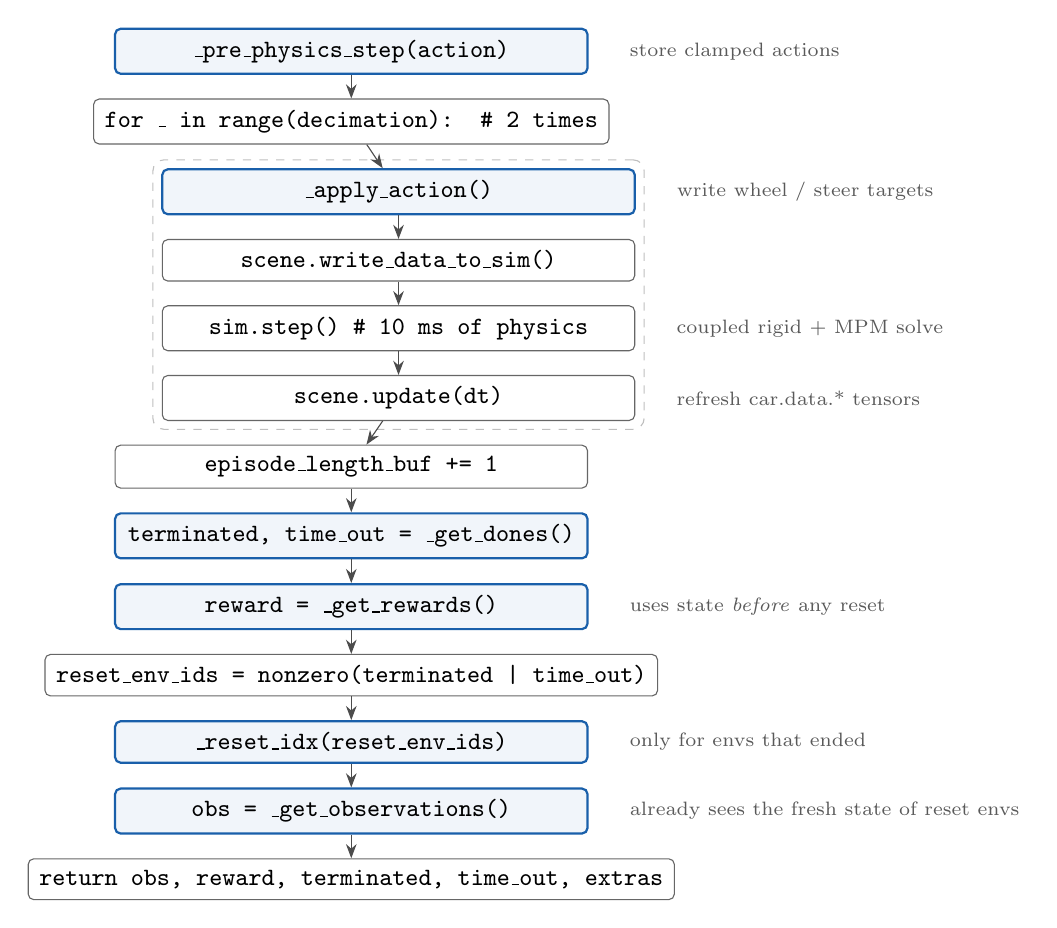
\begin{tikzpicture}[
  node distance=3mm,
  st/.style={draw,rounded corners=2pt,font=\small\ttfamily,inner sep=4pt,minimum width=6.0cm,align=left,fill=white},
  ours/.style={st,draw=isaacblue,thick,fill=isaacblue!6},
  lab/.style={st,draw=black!60},
  note/.style={font=\scriptsize,text=black!65,align=left},
  arr/.style={-{Stealth[length=1.8mm]},black!70}
]
\node[ours] (pre) {\_pre\_physics\_step(action)};
\node[note,right=4mm of pre] {store clamped actions};
\node[lab,below=of pre] (loop) {for \_ in range(decimation):   \# 2 times};
\node[ours,below=of loop,xshift=6mm] (apply) {\_apply\_action()};
\node[note,right=4mm of apply] {write wheel / steer targets};
\node[lab,below=of apply] (wds) {scene.write\_data\_to\_sim()};
\node[lab,below=of wds] (simstep) {sim.step()   \# 10 ms of physics};
\node[note,right=4mm of simstep] {coupled rigid + MPM solve};
\node[lab,below=of simstep] (upd) {scene.update(dt)};
\node[note,right=4mm of upd] {refresh car.data.* tensors};
\node[lab,below=of upd,xshift=-6mm] (cnt) {episode\_length\_buf += 1};
\node[ours,below=of cnt] (dones) {terminated, time\_out = \_get\_dones()};
\node[ours,below=of dones] (rew) {reward = \_get\_rewards()};
\node[note,right=4mm of rew] {uses state \emph{before} any reset};
\node[lab,below=of rew] (ids) {reset\_env\_ids = nonzero(terminated | time\_out)};
\node[ours,below=of ids] (reset) {\_reset\_idx(reset\_env\_ids)};
\node[note,right=4mm of reset] {only for envs that ended};
\node[ours,below=of reset] (obs) {obs = \_get\_observations()};
\node[note,right=4mm of obs] {already sees the fresh state of reset envs};
\node[lab,below=of obs] (ret) {return obs, reward, terminated, time\_out, extras};
\draw[arr] (pre) -- (loop);
\draw[arr] (loop) -- (apply);
\draw[arr] (apply) -- (wds);
\draw[arr] (wds) -- (simstep);
\draw[arr] (simstep) -- (upd);
\draw[arr] (upd) -- (cnt);
\draw[arr] (cnt) -- (dones);
\draw[arr] (dones) -- (rew);
\draw[arr] (rew) -- (ids);
\draw[arr] (ids) -- (reset);
\draw[arr] (reset) -- (obs);
\draw[arr] (obs) -- (ret);
\begin{scope}[on background layer]
\node[draw=black!25,dashed,rounded corners,fit=(apply)(wds)(simstep)(upd),inner sep=3pt] {};
\end{scope}
\end{tikzpicture}
\caption{Order of operations in \code{DirectRLEnv.step}. Blue: methods implemented in \code{tricycle_env.py}. The dashed group runs \code{decimation} times per call.}
\label{fig:step}
\end{figure}

Three consequences that the tricycle code relies on:

\begin{itemize}[leftmargin=1.6em]
  \item \textbf{Rewards are computed before resets.} \code{_get_rewards} may
        compare the current car position with the position stored last step
        (\code{_prev_x}); at that moment no env has been teleported yet.
  \item \textbf{Observations are computed after resets.} The observation
        returned for an env that just ended already describes the
        \emph{new} episode. \code{rsl_rl} knows the episode boundary from
        \code{dones}, so this is the expected behaviour.
  \item \textbf{\code{_apply_action} runs every physics sub-step,}
        \code{_pre_physics_step} once per control step. Cheap work (writing
        targets) belongs in the former, decoding the action in the latter.
\end{itemize}

\begin{isaacbox}{the Newton fast path for decimation}
After \code{sim.reset()}, \code{DirectRLEnv} asks the physics manager whether
it can run the whole decimation loop itself
(\srcpath{physics_manager.set_decimation(...)} /
\srcpath{handles_decimation()}). When it can, the loop in
Figure~\ref{fig:step} collapses into a single \code{sim.step} that internally
performs \code{decimation} physics steps under one CUDA graph, and
\code{_apply_action()} is called once. The observable behaviour for our task
is identical because \code{_apply_action} writes the same targets each time.
\end{isaacbox}

\section{Play}
\label{sec:play}

\begin{lstlisting}[style=shell]
.\isaaclab.bat play --rl_library rsl_rl --task Luna-Tricycle-Direct --num_envs 1 --checkpoint latest --viz newton
\end{lstlisting}

\code{play} follows the same path with two differences. First,
\code{hydra_task_config(..., play_mode=True)} calls
\code{env_cfg.play_mode()} after the presets are resolved and before scalar
overrides, so our override in \code{TricycleEnvCfg} caps the env count and
switches on particle rendering (Chapter~\ref{ch:env_cfg}); \code{--num_envs 1}
then still wins because it is applied afterwards. Second, instead of learning,
\code{play_rsl_rl.py} resolves the checkpoint (\code{latest} means the newest
run directory under \srcpath{logs/rsl_rl/tricycle} and its highest-numbered
\code{model_*.pt}), loads it into the runner, takes
\srcpath{runner.get_inference_policy()} (the deterministic mean action), exports
the network to \srcpath{exported/policy.pt} and \code{policy.onnx}, and loops
\code{obs, _, dones, _ = env.step(policy(obs))} until the window closes.

\code{--viz newton} attaches the Newton OpenGL visualiser. It draws rigid
shapes by default; soil particles are drawn only because our
\code{play_mode()} sets \code{show_particles=True}.

\chapter{The physics stack}
\label{ch:physics}

The tricycle runs on \textbf{Newton}, NVIDIA's GPU physics engine built on
Warp. Isaac Lab talks to Newton through a \emph{physics manager}, and the
tricycle uses two of Newton's solvers at once: a rigid-body solver for the car
and an implicit Material Point Method (MPM) solver for the soil. This chapter
explains the pieces that \code{tricycle_env_cfg.py} assembles, so that the
config in Chapter~\ref{ch:env_cfg} reads as a list of decisions rather than
magic numbers.

\section{Layers}

\begin{figure}[H]
\centering
\begin{tikzpicture}[
  layer/.style={draw,rounded corners=2pt,text width=13.2cm,minimum height=8mm,font=\footnotesize,align=center,fill=white},
  arr/.style={-{Stealth[length=1.8mm]},black!70}
]
\node[layer,fill=isaacblue!6,draw=isaacblue] (env) {\textbf{TricycleEnv / DirectRLEnv} \quad your methods + step bookkeeping};
\node[layer,below=3mm of env,fill=isaacblue!6,draw=isaacblue] (scene) {\textbf{InteractiveScene, Articulation, RigidObject, MPMObject} \quad tensors: \code{car.data.*}, \code{soil.data.*}};
\node[layer,below=3mm of scene,fill=isaacblue!6,draw=isaacblue] (sim) {\textbf{SimulationContext} \quad owns the stage and the physics manager};
\node[layer,below=3mm of sim,fill=newtonpurple!6,draw=newtonpurple] (mgr) {\textbf{NewtonCouplerManager} (\srcpath{isaaclab_contrib.coupling}) \quad builds one Newton Model, splits it into entries};
\node[layer,below=3mm of mgr,fill=newtonpurple!6,draw=newtonpurple] (solver) {\textbf{Newton SolverCoupledProxy} \quad entry ``rover'': SolverMuJoCo (MJWarp) \quad entry ``soil'': SolverImplicitMPM};
\node[layer,below=3mm of solver,fill=newtonpurple!6,draw=newtonpurple] (warp) {\textbf{Warp kernels on the GPU} \quad CUDA graph captured once, replayed every step};
\draw[arr] (env) -- (scene); \draw[arr] (scene) -- (sim); \draw[arr] (sim) -- (mgr); \draw[arr] (mgr) -- (solver); \draw[arr] (solver) -- (warp);
\end{tikzpicture}
\caption{From environment code to GPU kernels. Blue layers are Isaac Lab; purple layers are Newton.}
\end{figure}

\begin{isaacbox}{physics managers}
Isaac Lab develop can drive several physics backends (PhysX, Newton,
OmniPhysX). \srcpath{SimulationCfg.physics} selects one by holding a
\code{PhysicsCfg} subclass; \code{NewtonCfg}
(\srcpath{source/isaaclab_newton/isaaclab_newton/physics/newton_manager_cfg.py})
selects Newton. Inside \code{NewtonCfg}, \code{solver_cfg} selects
\emph{which} Newton solver manager runs the model: \code{MJWarpSolverCfg},
\code{MPMSolverCfg}, \code{XPBDSolverCfg}, \ldots, or, as here, a
\code{CouplerProxyCfg} from \srcpath{isaaclab_contrib.coupling} that nests two of
them. \srcpath{NewtonCfg.__post_init__} copies the manager class from
\srcpath{solver_cfg.class_type} so you never set it yourself.
\end{isaacbox}

\section{The rigid-body side: MuJoCo-Warp}

The car is an \emph{articulation}: a tree of rigid bodies (chassis, fork,
three wheels) connected by joints (one free joint for the chassis, one steering
hinge, three wheel hinges). Newton simulates it with \textbf{MJWarp}, a
GPU port of MuJoCo's dynamics. Isaac Lab wraps it as \code{MJWarpSolverCfg}
(\srcpath{physics/mjwarp_manager_cfg.py}). The four options the config sets:

\begin{description}[leftmargin=1.6em,font=\ttfamily]
  \item[use\_mujoco\_contacts=False] MuJoCo normally detects and resolves its
    own contacts. Setting this to \code{False} hands collision detection to
    Newton's own \emph{collision pipeline}, which is required whenever a
    Newton \code{collision_cfg} is also given (the two are mutually
    exclusive) and is what lets the coupler share contacts between solvers.
  \item[integrator="implicitfast"] MuJoCo's implicit-in-velocity integrator.
    It damps stiff joint drives and contacts far better than plain Euler at
    the same step size, which matters with a 10~ms step and velocity-driven
    wheels.
  \item[njmax=128] maximum number of constraint rows per env (joint limits,
    contacts, friction cones). Too small and contacts are dropped with a
    warning; too large only costs memory.
  \item[nconmax=128] maximum number of contact points per env.
\end{description}

\begin{isaacbox}{implicit actuators and \srcpath{use_newton_actuators}}
Our joints use \code{ImplicitActuatorCfg}. ``Implicit'' means the drive is a
PD controller \emph{inside the physics solver}: you give a position target
(steering) or a velocity target (rear wheels) plus \code{stiffness} and
\code{damping}, and the solver computes the torque as part of its implicit
step. \code{effort_limit_sim} and \code{velocity_limit_sim} are written into
the simulator as hard limits. \code{sim.use_newton_actuators = True} asks
Newton to author and execute these drives natively rather than through the
host-side adapter used for PhysX.
\end{isaacbox}

\section{The soil side: implicit MPM}
\label{sec:mpm}

\begin{newtonbox}{what MPM is}
The Material Point Method represents a continuum (soil, snow, mud) as a
cloud of \textbf{particles} that carry mass, velocity and deformation
history, plus a background \textbf{grid} on which forces are solved each
step. Every step: particle quantities are transferred to the grid
(``P2G''), the momentum equations with the material's constitutive law are
solved on the grid, and grid velocities are transferred back to move the
particles (``G2P''). Rigid bodies enter as \emph{colliders}: signed-distance
boundaries the grid velocities must respect. Newton's solver is
\emph{implicit}: it solves the yield condition as an optimisation problem
each step, which allows large steps (our 10~ms) without exploding.
\end{newtonbox}

Isaac Lab exposes it as \code{MPMSolverCfg}
(\srcpath{physics/mpm_manager_cfg.py}). The fields the tricycle sets, grouped:

\paragraph{Grid.}
\code{voxel_size=0.05} is the grid spacing (5~cm). \code{grid_type="sparse"}
allocates grid cells only where particles are. \code{grid_padding=0} adds no
empty margin. \srcpath{separate_worlds=True} gives every env its own grid so
envs cannot touch each other's soil and particle arrays are laid out
contiguously per env.

\paragraph{Sparse-grid capacities.}
\srcpath{max_active_cell_count}, \code{max_leaf_node_count},
\srcpath{max_lower_node_count}, \srcpath{max_upper_node_count} pre-allocate the
sparse tree (leaf $\to$ lower $\to$ upper nodes) so that the CUDA graph can
be captured once. They are \emph{totals across all envs}, not per env. Newton
requires \code{upper <= lower <= leaf <= active}. The committed values
$2^{14}/2^{13}/2^{12}/2^{10}$ were found by hand for 4 envs on 6~GB; a
``capacity exceeded'' error names the tier to raise, and a
``Failed to create volume'' plus CUDA error 700 means the caps were raised
too far for the memory available.

\paragraph{Numerics.}
\code{max_iterations=24} and \code{tolerance=1e-4} bound the per-step
rheology solve. \code{solver="auto"} lets Newton pick Gauss--Seidel for the
\code{Q1} velocity basis. \srcpath{warmstart_mode="auto"} reuses last step's
solution as a starting guess. \code{strain_basis="P0"} (piecewise constant
strain per cell), \code{velocity_basis="Q1"} (trilinear velocities) and
\srcpath{transfer_scheme="apic"} (affine particle-in-cell transfers, less
numerical damping than PIC) are the standard granular preset also used by
Isaac Lab's own \code{ur10_particle_push} task.

\paragraph{Colliders.}
\srcpath{collider_basis="pic27"} samples collider velocities with a 27-point
stencil; \srcpath{collider_velocity_mode="forward"} uses the colliders'
velocities at the start of the step. \srcpath{project_outside_colliders=False}
is mandatory on a coupled entry: it disables a particle-level push-out pass
that would fight the coupler.

\paragraph{The material.}
Particles carry an \code{MPMParticleMaterialCfg}
(\srcpath{sim/spawners/mpm/mpm_cfg.py}). Its fields: \code{density}
[kg/m$^3$], \code{young_modulus} [Pa], \code{poisson_ratio},
\code{viscosity} [Pa$\cdot$s], \code{friction} (dimensionless, $\approx
\tan\phi$ of the internal friction angle), \code{damping} [s],
\code{yield_pressure} [Pa], \code{tensile_yield_ratio}, \code{yield_stress}
[Pa] (cohesion), \code{hardening}, \code{dilatancy}. The yield surface is
\[
  \tau_{\max}(p) \;=\; \texttt{yield\_stress} \;+\; \texttt{friction}\cdot(p - p_{\min}),
\]
so shear strength grows with pressure $p$ like dry sand. The tricycle soil
sets \code{density=1800}, \code{friction=0.84} ($=\tan 40^\circ$) and
\code{yield_pressure=1e12} (effectively incompressible), leaving the very
stiff default \code{young_modulus} so the strip behaves like packed ground
rather than a sandbox.

\paragraph{The particles.}
\code{MPMGridCfg} fills an axis-aligned box with a lattice. Its resolution
per axis is $\lceil \texttt{particles\_per\_cell}\cdot \text{extent}/\texttt{voxel\_size}\rceil$,
so the $1.5\times0.6\times0.06$~m strip at 5~cm voxels gives $30\times12\times2 = 720$
particles per env, each placed at a cell centre
(\srcpath{particle_placement="cell_center"}) with mass = cell volume $\times$
density.

\begin{whybox}{the soil needs its own floor}
The MPM solver only sees colliders that belong to \emph{its} coupler entry.
The world ground plane belongs to the rigid entry, so to the soil it does not
exist and particles would fall forever. \code{tricycle_env_cfg.py} therefore
adds \code{MPMGround}, an invisible kinematic slab just below the strip, and
lists it as the MPM entry's only body.
\end{whybox}

\section{Coupling the two solvers}
\label{sec:coupling}

\begin{newtonbox}{one Newton model, two solvers}
Newton's experimental \emph{coupled solver} takes a single \code{Model} and a
list of \textbf{entries}. Each entry owns a subset of bodies, joints, shapes
and particles (a \code{ModelView}) and runs its own solver on that subset.
\textbf{Proxy mappings} expose selected bodies of one entry inside another
as \emph{virtual proxies}: massive ghost bodies whose pose is copied from the
source each step and whose accumulated contact impulses are sent back as
feedback forces. Newton calls this \emph{lagged-impulse} coupling because the
feedback is applied one step late.
\end{newtonbox}

Isaac Lab wraps this as \code{CouplerProxyCfg}
(\srcpath{source/isaaclab_contrib/isaaclab_contrib/coupling/coupler_cfg.py}):

\begin{itemize}[leftmargin=1.6em]
  \item \code{entries}: a list of \code{CouplerEntryCfg}. Each has a
        \code{name}, a \code{solver_cfg}, a list of \code{bodies} (regexes
        matched against full Newton body labels, descendants included),
        \code{all_particles}, \srcpath{include_static_shapes} (whether the entry
        owns shapes with no body, such as the ground plane),
        \srcpath{include_child_joints}, \code{substeps} (how many equal
        sub-steps the entry takes inside one coupled step) and
        \code{in_place} (step into the same state buffer; required
        \code{True} for MPM).
  \item \code{proxies}: a list of \code{CouplerProxyMappingCfg} with
        \code{source}, \code{destination}, \code{bodies},
        \code{mode} (\code{"lagged"} or \code{"staggered"}), \srcpath{mass_scale} and
        \code{collision_pipeline}.
  \item \code{iterations}: proxy relaxation passes per coupled step.
\end{itemize}

\begin{figure}[H]
\centering
\begin{tikzpicture}[
  ent/.style={draw,rounded corners=3pt,minimum width=5.6cm,minimum height=2.6cm,align=left,font=\small,fill=white},
  arr/.style={-{Stealth[length=2mm]},thick},
]
\node[ent,draw=isaacblue,fill=isaacblue!5] (rig) at (0,0) {\textbf{entry ``rover''} (MJWarp, 2 substeps)\\[2pt]
  bodies: \srcpath{/World/envs/env_.*/Tricycle}\\ + all static shapes (ground plane)\\[2pt] solves: car dynamics, wheel drives,\\ car vs ground contacts};
\node[ent,draw=newtonpurple,fill=newtonpurple!5] (mpm) at (7.6,0) {\textbf{entry ``soil''} (implicit MPM, 1 substep)\\[2pt]
  bodies: \srcpath{/World/envs/env_.*/MPMGround}\\ + all particles\\[2pt] solves: soil flow, soil vs slab,\\ soil vs \emph{proxy} wheels};
\draw[arr,isaacblue] ([yshift=5mm]rig.east) -- node[above,font=\scriptsize,align=center]{proxy: wheel poses \& velocities\\ (mass $\times$ 10)} ([yshift=5mm]mpm.west);
\draw[arr,newtonpurple] ([yshift=-5mm]mpm.west) -- node[below,font=\scriptsize,align=center]{lagged feedback: soil impulses\\ on the wheels, next step} ([yshift=-5mm]rig.east);
\end{tikzpicture}
\caption{The two coupler entries and the one proxy mapping in \code{TricycleEnvCfg.__post_init__}. Only the three wheel bodies are mirrored into the soil solver.}
\label{fig:coupler}
\end{figure}

What happens each 10~ms physics step: the rigid entry advances the car by two
5~ms sub-steps using last step's soil feedback; the wheels' new poses and
velocities are copied onto their proxies inside the MPM view; the MPM entry
advances the soil one 10~ms step, colliding particles against the proxy
wheels and the slab; the impulses the particles exerted on the proxies are
stored and applied to the real wheels during the \emph{next} rigid step.

\begin{whybox}{\code{mass_scale} is the stability knob}
A proxy body is given the source body's mass times \code{mass_scale}. A
heavy proxy barely moves when soil pushes on it, so the soil solve stays
well-posed and the feedback impulses are smooth; the real wheel then receives
those impulses one step late. If the scale is too small the lagged feedback
can oscillate (the car ``chatters'' on the strip); too large and the soil
feels the wheel as an immovable wall. The tricycle uses 10 through
\srcpath{TricycleEnvCfg.proxy_mass_scale}.
\end{whybox}

\begin{warnbox}{rules the coupler enforces}
\begin{itemize}[leftmargin=1.4em,nosep]
  \item An MPM entry must have \code{in_place=True}; the coupler raises
        \code{ValueError} otherwise (\code{coupler.py}, \code{_validate_config}).
  \item A proxy \emph{source} entry may not be \code{in_place} in lagged mode
        (Newton, \srcpath{solver_coupled_proxy.py}). The rigid entry is not, so
        this is satisfied.
  \item \srcpath{project_outside_colliders} must be \code{False} on a coupled
        MPM entry.
  \item Newton's proxy coupler supports at most two entries.
\end{itemize}
\end{warnbox}

\section{The collision pipeline and \texttt{soft\_contact\_max=0}}

With \srcpath{use_mujoco_contacts=False}, rigid contacts (car against ground
plane) come from Newton's \code{CollisionPipeline}, configured by
\code{NewtonCollisionPipelineCfg} (\srcpath{physics/newton_collision_cfg.py}).
The only field the tricycle sets is \code{soft_contact_max=0}. ``Soft
contacts'' are particle-versus-shape contacts generated by the generic
pipeline; their default allocation is \code{shape_count * particle_count},
which for thousands of particles is a huge buffer, and the MPM solver handles
particle contacts itself anyway. Setting the maximum to zero disables that
allocation.

\section{Time stepping and CUDA graphs}

\code{SimulationCfg.dt = 1/100} is the physics step; \srcpath{NewtonCfg.num_substeps=1}
means one coupled solve per step (the rigid entry's own \code{substeps=2}
happens inside it). \code{use_cuda_graph=True} records the whole step as a
CUDA graph the first time and replays it afterwards, which is where most of
the speed comes from; it also explains why buffer sizes (grid capacities,
\code{njmax}) must be fixed up front. \code{decimation=2} in the env cfg
means the policy acts every second physics step, i.e.\ at 50~Hz.

\section{Why only a handful of envs fit}

Each env carries 720 particles plus its own sparse grid; the grid tiers are
shared caps. The GPU work per step is dominated by the number of \emph{active
grid cells} times envs, and the 6~GB card runs out of memory well before the
GPU runs out of compute. The runbook's numbers (4 envs, 90--160 steps/s) are
the practical ceiling for this card; the same configuration on a large GPU
simply needs the four caps raised in proportion to \code{--num_envs}.

\chapter{From MJCF to USD: the car asset}
\label{ch:asset}

The car is described twice in the repository: once as MJCF text inside
\code{tricycle.py}, and once as a set of USD files under
\srcpath{assets/tricycle/}. Only the USD is loaded at run time. This chapter
explains how one becomes the other and what each USD layer contains, so that
Chapters~\ref{ch:tricycle_py} and \ref{ch:usd} can go line by line.

\section{Why two descriptions}

MJCF (MuJoCo's XML format) is compact and human-writable: a body, a joint, a
geom, done. Isaac Lab's Newton backend, however, builds its physics model from
the \emph{USD stage} that \code{InteractiveScene} spawns. Isaac Lab can convert
MJCF to USD, but the importer it uses is a Kit extension that only exists
inside a running Isaac Sim application; the \code{isaaclab train} command never
starts Kit. So the conversion is done once, offline, with
\srcpath{scripts/tools/convert_mjcf.py}, and the result is committed.

\begin{warnbox}{stale assets}
Nothing checks that \srcpath{assets/tricycle/} matches \code{tricycle.py}. If
you edit the MJCF and forget to reconvert, training silently uses the old car.
The runbook's ``Convert the tricycle asset'' step is the fix, and
\code{tricycle.py} now says so in its header. For this revision the committed
USD was regenerated to match the new body.
\end{warnbox}

\section{Anatomy of the MJCF}

\begin{lstlisting}[style=plain,numbers=none]
<mujoco model="tricycle">
  <compiler .../>          units and options for MuJoCo's model compiler
  <default> ... </default> attributes every geom / joint inherits unless overridden
  <worldbody>
    <body name="chassis">  a rigid body; pos is relative to its parent
      <freejoint/>         6 degrees of freedom: the chassis floats
      <geom .../>          a shape with mass, attached to the body
      <body name="fork">   a child body; its pos is relative to chassis
        <joint .../>       1 degree of freedom between fork and chassis
        ...
\end{lstlisting}

Bodies form a tree. Each body's pose is given relative to its parent, each
joint sits between a body and its parent, and each geom belongs to exactly one
body. Mass and inertia of a body are the sums over its geoms (MuJoCo computes
the inertia tensor of a box or sphere from its dimensions and the given mass).
That is why every body in \code{tricycle.py} has at least one geom with a
mass: a body with zero inertia makes the solver divide by zero.

\section{The converter}

\code{convert_mjcf.py} wraps \srcpath{isaaclab.sim.converters.MjcfConverter}.
On the develop branch this converter drives the \emph{MuJoCo USD Converter}
(the \code{customLayerData} of every output file says
\code{"MuJoCo USD Converter v0.2.0"}), which compiles the MJCF with MuJoCo's
own compiler and then writes USD prims for what it finds. Isaac Lab then runs
two post-processing passes recorded in \srcpath{assets/config.yaml}:
\srcpath{run_asset_transformer} adds the Isaac robot schemas
(\code{IsaacRobotAPI}, \code{IsaacLinkAPI}, \code{IsaacJointAPI}), and
\srcpath{run_multi_physics_conversion} splits the physics into selectable
variants (\code{physics}, \code{mujoco}, \code{physx}, \code{none}).

The output is a small tree of \code{.usda} files (USD's text format):

\begin{center}
\small
\begin{tabular}{@{}ll@{}}
\toprule
File & Contains \\
\midrule
\code{tricycle.usda} & the entry point: references \code{base.usda}, defines the \code{Physics} variant set \\
\srcpath{payloads/base.usda} & the geometry: one \code{Xform} per body, one \code{Cube}/\code{Sphere}/\code{Capsule} per geom \\
\srcpath{payloads/robot.usda} & Isaac robot/link/joint tags, sublayered into \code{base.usda} \\
\srcpath{payloads/Physics/physics.usda} & rigid-body, articulation-root, collision and mass schemas; the joints \\
\srcpath{payloads/Physics/mujoco.usda} & MuJoCo-only extras (\code{MjcJointAPI} with \code{mjc:damping}) \\
\srcpath{payloads/Physics/physx.usda} & PhysX-only extras (\code{PhysxJointAPI}); unused with Newton \\
\bottomrule
\end{tabular}
\end{center}

\begin{isaacbox}{USD in five sentences}
A USD \emph{stage} is a tree of \emph{prims} (nodes) each with a type
(\code{Xform}, \code{Cube}, \code{PhysicsRevoluteJoint}, \ldots) and
attributes. \emph{API schemas} such as \code{PhysicsRigidBodyAPI} are tags that
can be applied to a prim to give it extra attributes and meaning. A stage is
\emph{composed} from several files: \code{def} creates a prim,
\code{over} adds to a prim defined elsewhere, \code{references} and
\code{payload} pull in other files, \code{subLayers} stack files. A
\emph{variant set} is a switch that selects which of several alternative
sub-trees is active; Isaac Lab leaves the \code{Physics} variant on
\code{"physics"}, so the \code{mujoco} and \code{physx} payloads are not
loaded. Newton reads the composed result: bodies from
\code{PhysicsRigidBodyAPI} prims, shapes from prims with
\code{PhysicsCollisionAPI}, masses from \code{PhysicsMassAPI}, joints from
\code{Physics*Joint} prims.
\end{isaacbox}

\section{How MJCF names become prim paths}
\label{sec:prim_paths}

The converter keeps the body tree and the body names:

\begin{lstlisting}[style=plain,numbers=none]
MJCF body tree                    USD prim (inside the asset)
chassis                           /tricycle/Geometry/chassis
  fork                            /tricycle/Geometry/chassis/fork
    front_wheel_body              /tricycle/Geometry/chassis/fork/front_wheel_body
  rear_left_body                  /tricycle/Geometry/chassis/rear_left_body
  rear_right_body                 /tricycle/Geometry/chassis/rear_right_body
joint "steer"                     /tricycle/Geometry/chassis/fork/steer
joint "front_wheel"               /tricycle/Geometry/chassis/fork/front_wheel_body/front_wheel
joint "rear_left"                 /tricycle/Geometry/chassis/rear_left_body/rear_left
\end{lstlisting}

When \code{InteractiveScene} spawns the asset at
\code{prim_path="{ENV_REGEX_NS}/Tricycle"}, the asset root
\srcpath{/tricycle} is placed at \srcpath{/World/envs/env_0/Tricycle},
\srcpath{/World/envs/env_1/Tricycle}, and so on. The full Newton body label of the
left rear wheel in env 0 is therefore
\srcpath{/World/envs/env_0/Tricycle/Geometry/chassis/rear_left_body}. This is
where two conventions in the env cfg come from:

\begin{itemize}[leftmargin=1.6em]
  \item Scene configs use the macro \code{{ENV_REGEX_NS}}, which Isaac Lab
        expands to \srcpath{/World/envs/env_.*}.
  \item Coupler \code{bodies} lists are plain regexes matched by Newton, so
        they spell the expansion out:
        \srcpath{/World/envs/env_.*/Tricycle/Geometry/chassis/.*_body} matches
        all three wheel bodies (the \code{.*} also swallows \srcpath{fork/}),
        but not the chassis or the fork.
\end{itemize}

Joint \emph{names} survive too: \srcpath{Articulation.find_joints(["steer"])}
works because the USD joint prim is called \code{steer}.

\section{What the new body looks like}
\label{sec:new_body}

The original chassis was a single $40\times24\times8$~cm box with the front
wheel poking out of its nose. It has been replaced by a triangular frame: two
side rails running from the steering head back to the rear corners, a rear
crossbar, and a flat deck inside the rear half. All four are box geoms; the
total chassis mass (5.0~kg), the wheel positions, radii and masses, and every
joint and body name are unchanged, so the env config and the coupler mapping
did not have to change.

\begin{figure}[H]
\centering
\begin{subfigure}[t]{0.48\textwidth}
  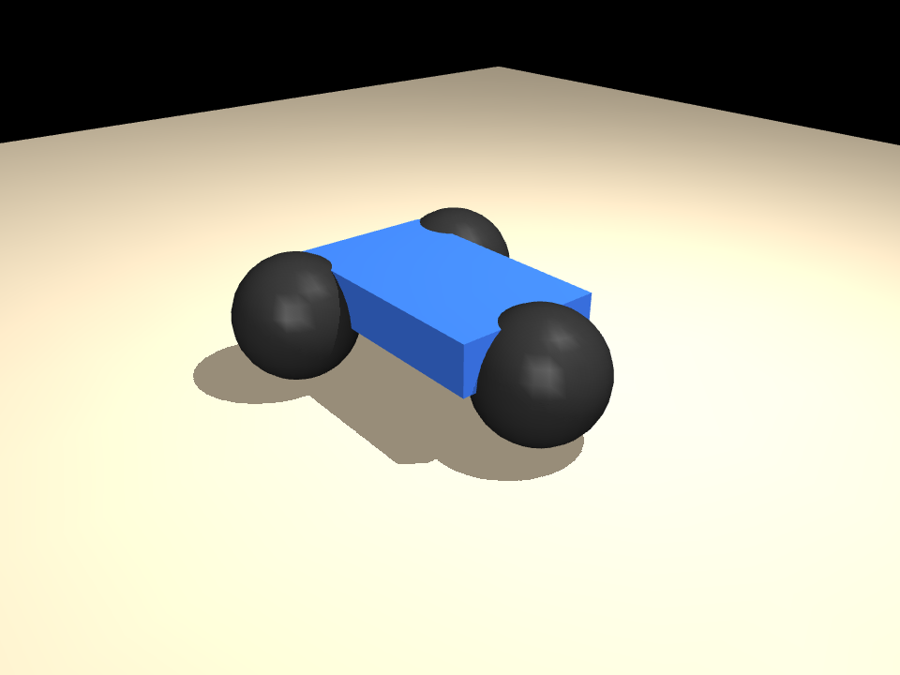
\includegraphics[width=\linewidth]{tricycle_old_iso}
  \caption{Before: box chassis.}
\end{subfigure}\hfill
\begin{subfigure}[t]{0.48\textwidth}
  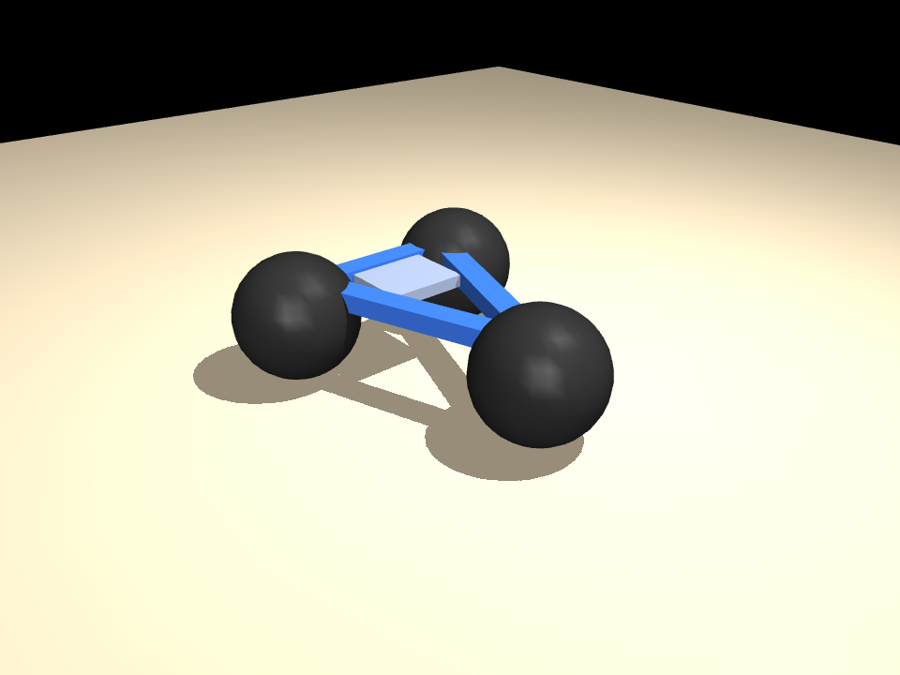
\includegraphics[width=\linewidth]{tricycle_new_iso}
  \caption{After: triangular frame with deck.}
\end{subfigure}
\\[6pt]
\begin{subfigure}[t]{0.48\textwidth}
  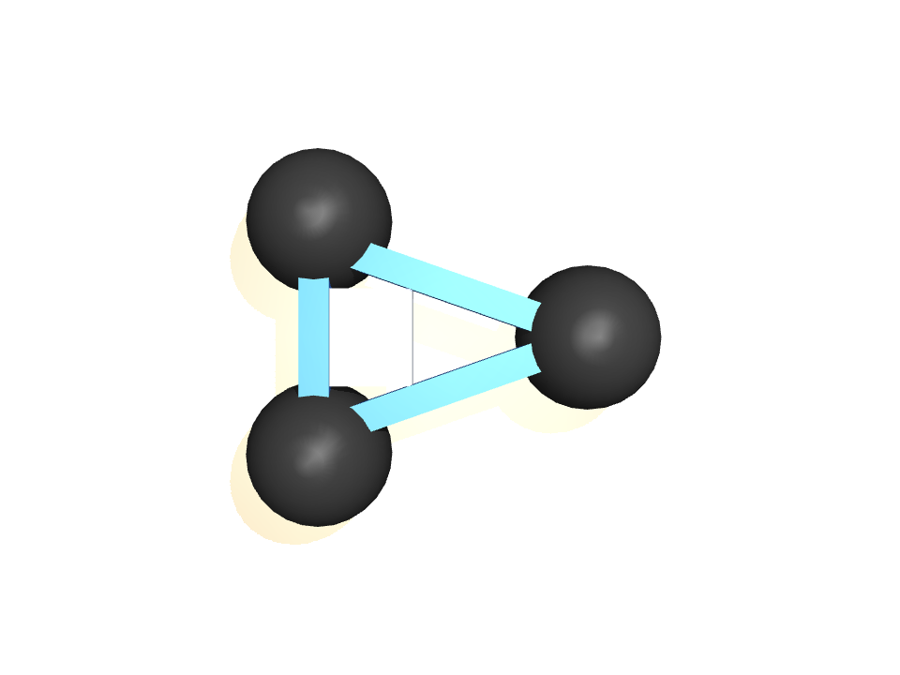
\includegraphics[width=\linewidth]{tricycle_new_top}
  \caption{After, plan view. Apex forward (right), rear wheels at the base.}
\end{subfigure}\hfill
\begin{subfigure}[t]{0.48\textwidth}
  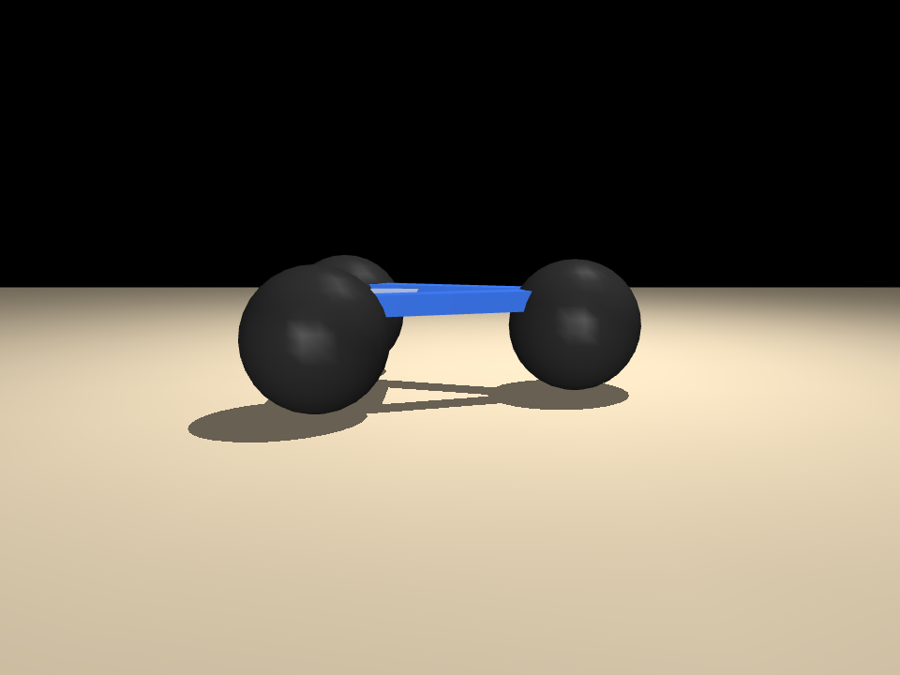
\includegraphics[width=\linewidth]{tricycle_new_side}
  \caption{After, side view. The frame sits at 14~cm, wheel centres at 10~cm.}
\end{subfigure}
\caption{The tricycle as compiled by MuJoCo from \code{tricycle.py} (rendered with MuJoCo's own renderer, not Isaac Lab).}
\label{fig:body}
\end{figure}

Because the wheels are 10~cm spheres and the frame sits at the chassis height
of 14~cm, the frame's three corners disappear inside the wheels: the rails
run into the rear wheels and the apex sits inside the front wheel. That is
intentional; the corners of a real tricycle frame are also hidden by its hubs.

\section{Regenerating the USD}

Whenever \code{tricycle.py} changes, run the two commands in
\code{RUNBOOK.md}, ``Convert the tricycle asset'': the first writes the MJCF
to a temp file with \code{write_mjcf()}, the second converts it. The converter
writes into \srcpath{assets/tricycle/tricycle.usda} regardless of the exact
output filename given, and updates \srcpath{assets/config.yaml} and
\srcpath{assets/.asset_hash}. Isaac Lab uses the hash to skip conversion when
neither the MJCF nor the converter settings changed
(\code{force_usd_conversion: true} in the committed config always
reconverts).

\part{Every file, every line}
\chapter{\texttt{pyproject.toml}}
\label{ch:pyproject}

\textbf{Role:} tells \code{pip} how to install the package and tells Isaac Lab
that the package contains tasks. It is read once, at install time
(Section~\ref{sec:when}). 17 lines.

\plainfile{\srcroot/pyproject.toml}

\begin{explain}
\li{1} Opens the \code{[project]} table, the standard place (PEP~621) for a
  package's metadata.
\li{2} The distribution name. This is what \code{pip list} shows and what the
  installed metadata folder is called (\srcpath{luna_hifi_tasks-0.1.0.dist-info}).
  It happens to equal the import name, but the two are independent.
\li{3} Version string; not used by anything in Isaac Lab, but required by pip.
\li{4} Free-text description shown by \code{pip show}.
\li{5} Refuses to install on Python older than 3.11. Newton~1.5 uses the
  \code{X | None} union syntax in type annotations at run time, which Python
  3.10 rejects (RUNBOOK section 1). The runbook goes further and uses 3.12.
\li{6} No dependencies are declared, deliberately. Isaac Lab, Newton, torch,
  warp and gymnasium all come from the Isaac Lab venv; declaring them here
  would make pip try to resolve versions it must not touch.
\li{7} Blank separator.
\li{8} Opens the entry-point table for the group \code{isaaclab.tasks}. The
  quotes are needed because the group name contains a dot. This is the single
  line that makes the package discoverable by the \code{isaaclab} command
  (Section~\ref{sec:step_cli}).
\li{9} One entry point: name \code{luna_hifi_tasks}, target the module
  \code{luna_hifi_tasks}. When Isaac Lab calls \code{entry_point.load()} on it,
  Python imports that module, which triggers the task registration. The
  target could have been a sub-module or an object; the whole package is used
  so that adding \code{from . import excavation} later registers the second
  task without touching this file.
\li{10} Blank.
\li{11} Opens the build-system table: which tool turns this folder into an
  installable package.
\li{12} Requires \code{setuptools} 64 or newer, the first version with
  PEP~660 editable installs. That is what makes \code{pip install -e} work
  without a \code{setup.py}.
\li{13} The build backend entry point inside setuptools.
\li{14} Blank.
\li{15} Configures setuptools' automatic package discovery.
\li{16} Search for packages starting in the repository root.
\li{17} Only take folders whose name starts with \code{luna_hifi_tasks}. This
  excludes \code{assets}, \code{docs} and anything else at the root. A
  folder only counts as a package if it contains \code{__init__.py}; a
  sub-folder without one is silently skipped, which is the
  missing-\code{__init__.py} failure mode in the runbook. Adding the file is
  the whole fix; see the box below on why no reinstall is needed for it.
\end{explain}

\begin{isaacbox}{editable installs, and when a reinstall is needed}
\code{pip install -e <folder>} does not copy the code. With a modern
setuptools (PEP~660) it writes two things into the venv's
\code{site-packages}: a \code{.pth} file that installs an import finder, and
the distribution metadata in \srcpath{luna_hifi_tasks-0.1.0.dist-info}. The
finder holds a single mapping, the top-level name \code{luna_hifi_tasks}
pointing at your source folder; every module below it is resolved off the
filesystem at import time.

So the source tree is read live, and \emph{one} kind of change needs a
reinstall: editing \code{pyproject.toml}. Entry points and the package list
are frozen into \code{dist-info} when you install, so a new or renamed entry
point stays invisible until \code{pip install -e} runs again. Everything else
takes effect on the next run: editing any \code{.py} file, adding a new
subpackage, and adding an \code{__init__.py} to a folder that lacked one.

The \srcpath{luna_hifi_tasks.egg-info/} folder that appears in the repository
root is a leftover of the build, not the metadata anything reads; deleting it
does not affect task discovery. All four behaviours were checked directly on
this package in a clean virtual environment.
\end{isaacbox}

\chapter{\texttt{luna\_hifi\_tasks/\_\_init\_\_.py}}
\label{ch:package_init}

\textbf{Role:} the package root. Importing it is what the Isaac Lab entry point
does at start-up; its only job is to import the sub-packages that register
tasks. 1 line.

\codefile{\srcroot/luna_hifi_tasks/__init__.py}

\begin{explain}
\li{1} A relative import of the \code{tricycle} sub-package. Python executes
  \srcpath{luna_hifi_tasks/tricycle/__init__.py} as a side effect, and that file
  registers \code{Luna-Tricycle-Direct} with Gymnasium
  (Chapter~\ref{ch:task_init}). The trailing \texttt{\# noqa: F401} tells linters
  that the ``unused import'' is intentional: nothing here uses the name
  \code{tricycle}, the import exists for its side effect.
  The \code{excavation} sub-package is \emph{not} imported, which is the
  concrete reason the two tasks are independent (Section~\ref{sec:independent}).
  When the excavation task is ready, a second line
  \texttt{from . import excavation  \# noqa: F401} registers it.
\end{explain}

\begin{warnbox}{a stray file that used to live at the repository root}
Until this revision the repository also contained a file literally named
\code{__init__ .py} (with a space) at the root, holding two import lines
including \code{excavation}. A file with a space in its name cannot be
imported, so it was dead; it has been deleted. The real package init is the
one-liner above.
\end{warnbox}

\chapter{\texttt{tricycle/\_\_init\_\_.py}: registering the task}
\label{ch:task_init}

\textbf{Role:} gives the task its public name and tells Gymnasium and Isaac
Lab which three classes implement it. Runs once at start-up. 25 lines.

\codepart{\srcroot/luna_hifi_tasks/tricycle/__init__.py}{1}{11}

\begin{explain}
\lis{1}{11} Header comment. Lines 3--5 state the mechanism (entry point
  $\to$ import $\to$ registration); lines 7--8 are the two commands from the
  runbook, so anyone opening the file sees how to run it; lines 10--11 give
  the success criterion in the unit the reward is measured in (metres in
  2~s).
\end{explain}

\codepart{\srcroot/luna_hifi_tasks/tricycle/__init__.py}{12}{25}

\begin{explain}
\li{13} Gymnasium is the maintained fork of OpenAI Gym. Isaac Lab uses its
  registry as the phone book of tasks; nothing else from it is needed here.
\li{15} Imports the \code{agents} sub-package so that \code{agents.__name__}
  can be used on line 23 to spell the dotted path of the PPO config
  without hard-coding it. This also executes \srcpath{agents/__init__.py}, which
  is empty.
\li{17} \code{gym.register} adds one entry to the global registry. Everything
  inside the call is stored as data; no class is imported yet.
\li{18} The task id. Isaac Lab develop's own tasks drop the \code{-v0} suffix
  the old scripts used, and so do we. \code{--task Luna-Tricycle-Direct}
  on the command line must match this string exactly.
\li{19} The environment class as a dotted path string,
  \code{module:ClassName}. \code{__name__} is \srcpath{luna_hifi_tasks.tricycle},
  so this reads \srcpath{luna_hifi_tasks.tricycle.tricycle_env:TricycleEnv}.
  Gymnasium imports it lazily when \code{gym.make} is called
  (Section~\ref{sec:step_env}).
\li{20} Gymnasium normally wraps every environment in a checker that
  validates observation shapes against the declared space on each step. Isaac
  Lab environments return dictionaries of batched tensors, which the checker
  does not understand, so every Isaac Lab task disables it.
\li{21} Extra keyword arguments. Gymnasium passes them to the environment
  constructor, but Isaac Lab reads them earlier, from the registry, to find
  the config classes.
\li{22} \code{env_cfg_entry_point}: the environment config class. Isaac Lab's
  \code{load_cfg_from_registry(task, "env_cfg_entry_point")} imports
  \srcpath{luna_hifi_tasks.tricycle.tricycle_env_cfg} and instantiates
  \code{TricycleEnvCfg} (Section~\ref{sec:step_cfg}).
\li{23} \srcpath{rsl_rl_cfg_entry_point}: the agent config for the
  \code{rsl_rl} library, built from \code{agents.__name__}
  (\srcpath{luna_hifi_tasks.tricycle.agents}) plus the module and class. The key
  name is a convention: \code{--rl_library rsl_rl} makes Isaac Lab look up
  \srcpath{rsl_rl_cfg_entry_point}; a \code{skrl} backend would look for
  \srcpath{skrl_cfg_entry_point}, and so on.
\li{24} Closes the \code{kwargs} dictionary.
\li{25} Closes the \code{gym.register} call.
\end{explain}

\begin{isaacbox}{the three classes behind one task id}
Every Isaac Lab task is a triple: an \emph{env class} (behaviour), an
\emph{env cfg class} (data: scene, physics, spaces), and one \emph{agent cfg
class per learning library}. The registry stores their import paths as
strings so that listing tasks does not import heavy modules. The
\code{gym.make} call and the two \srcpath{load_cfg_from_registry} calls are where
the strings are turned into classes.
\end{isaacbox}

\chapter{\texttt{tricycle.py}: the car model}
\label{ch:tricycle_py}

\textbf{Role:} defines the car as an MJCF string and offers a helper to write
it to disk for conversion. At run time only three constants are imported from
it (\code{CHASSIS_Z}, \code{JOINT_STEER}, \code{JOINT_REAR}); the MJCF itself
is used offline (Chapter~\ref{ch:asset}). 156 lines.

\section{Header}

\codepart{\srcroot/luna_hifi_tasks/tricycle/tricycle.py}{1}{29}

\begin{explain}
\lis{1}{4} What the file is.
\lis{6}{9} The most important operational fact about this file: it is
  \emph{not} read during training. The USD under \srcpath{assets/} is, and it
  must be regenerated when this file changes.
\lis{11}{18} An ASCII plan view of the body so that the numbers below have a
  picture: the two rails meet at the apex over the front wheel; the crossbar
  closes the rear; the deck sits inside.
\lis{20}{23} Why the wheels are spheres. The implicit MPM solver treats
  colliders as signed-distance fields; a sphere's distance function is one
  subtraction and one square root, the cheapest and most robust collider it
  has. For ``does the pipeline train'' the shape of the contact patch does
  not matter. Line 22--23 records that wheel positions and radii were kept
  from the first working version so the soil coupling did not move.
\lis{25}{26} A body whose geoms have zero total mass has a zero inertia
  tensor, and the solver divides by it. Every body here carries a geom with an
  explicit \code{mass}.
\lis{28}{29} The coordinate convention: $+x$ forward, $+z$ up, wheel bottoms
  at $z=0$ when the chassis origin is at $z=0.14$.
\end{explain}

\section{Imports and dimensions}

\codepart{\srcroot/luna_hifi_tasks/tricycle/tricycle.py}{31}{66}

\begin{explain}
\li{31} Lets the annotations on line 73 (\code{str | None},
  \code{tuple[float, float]}) be written in the modern form on any Python
  3.7+.
\lis{33}{35} \code{math} for the rail geometry, \code{os} and
  \code{tempfile} for \code{write_mjcf}.
\li{41} Sphere radius of all three wheels, 10~cm.
\li{42} Height of the chassis body origin above the ground when the wheels
  rest on $z=0$. \code{tricycle_env_cfg.py} imports this to compute the spawn
  height.
\li{43} Wheel centres relative to the chassis origin: $0.10 - 0.14 = -0.04$.
  Defined once so the three wheel bodies cannot drift apart.
\li{45} $x$ of the steering axis and the front wheel centre, 22~cm ahead of
  the chassis origin.
\li{46} $x$ of the rear axle, 15~cm behind. Wheelbase $= 0.37$~m.
\li{47} Half the rear track: rear wheel centres at $y=\pm0.16$.
\li{50} The apex of the triangle, directly over the steering axis.
\li{51} The rear corners of the triangle sit at $y=\pm0.13$, 3~cm inside the
  wheel centres, so the rails end inside the wheel spheres and the corners
  are visually capped by the wheels (Section~\ref{sec:new_body}).
\lis{52}{53} Rail cross-section: half-width 2~cm, half-height 1.5~cm, i.e.\
  4~cm wide and 3~cm tall. MuJoCo box sizes are always half-extents.
\lis{56}{58} Geom masses. $0.8 + 0.8 + 0.8 + 2.6 = 5.0$~kg, the same as the
  old single box, so the car's weight, wheel loads and drive torques are
  unchanged. Compiled with MuJoCo, the chassis centre of mass lands at
  $x=-0.054$~m (slightly behind the origin, towards the driven wheels) and
  the principal inertia is about $(0.062, 0.044, 0.019)$~kg\,m$^2$.
\lis{60}{62} Joint names. These strings appear in the MJCF, survive the USD
  conversion as prim names, and are what \code{tricycle_env.py} passes to
  \code{find_joints}. \code{JOINT_REAR} is a list because the two rear wheels
  are always addressed together.
\lis{64}{66} Colours as MJCF \code{rgba} strings. The converter copies them
  into \code{primvars:displayColor}, so they are what the Newton viewer
  shows.
\end{explain}

\section{Building the frame}

\codepart{\srcroot/luna_hifi_tasks/tricycle/tricycle.py}{68}{99}

\begin{explain}
\li{73} A helper that returns one \code{<geom>} element for a box whose local
  $x$ axis runs from \code{start} to \code{end} in the chassis $xy$-plane.
  Writing the rails this way means the numbers are derived from the corner
  coordinates rather than typed by hand.
\li{74} Docstring.
\li{75} The vector from start to end.
\li{76} Half the rail length; MuJoCo wants half-extents. For the rails,
  $\tfrac12\sqrt{0.37^2+0.13^2} = 0.1961$~m.
\li{77} The yaw angle of that vector. For the left rail (from $(-0.15,
  0.13)$ to $(0.22, 0)$) it is $\operatorname{atan2}(-0.13, 0.37) =
  -0.338$~rad $\approx -19.4^\circ$; the right rail gets $+0.338$.
\li{78} The rail's centre: the midpoint, $(0.035, \pm0.065)$.
\lis{79}{82} Emit the element. \code{pos} is the centre, \code{euler="0 0
  yaw"} rotates about $z$ (the compiler is told on line 107 that angles are
  radians), \code{size} is (half-length, half-width, half-height),
  \code{mass} fixes the mass (MuJoCo derives the density and the inertia),
  \code{rgba} the colour. The \code{name} lets the geom be found in the USD.
\li{85} The left rail: from the left rear corner to the apex.
\li{86} The right rail: mirror image.
\lis{89}{93} The crossbar, a box centred on the rear axle line
  ($x=-0.15$), half-length in $y$ of $0.13+0.02 = 0.15$ so that it covers
  the rails' ends, and the same cross-section as the rails.
\lis{96}{99} The deck: a $12\times13\times2$~cm plate centred at
  $x=-0.08$, i.e.\ filling the rear half of the triangle where it is wide
  enough, 5~mm lower than the rails' top surface so it reads as a floor pan.
  It carries 2.6 of the 5~kg.
\end{explain}

\begin{whybox}{why boxes and not a triangular mesh}
MJCF has no triangle primitive. A mesh with inline vertices would survive
MuJoCo's compiler, but boxes are the safest shape for every stage of the
pipeline: the USD converter writes them as \code{Cube} prims with a scale,
Newton's rigid collision pipeline handles boxes analytically, and the Isaac
Lab visualiser draws them without any mesh import. Three rails plus a deck
give an unmistakable triangle at zero risk.
\end{whybox}

\section{The MJCF string}

\codepart{\srcroot/luna_hifi_tasks/tricycle/tricycle.py}{101}{143}

\begin{explain}
\li{105} An f-string: every \code{{...}} is filled in by Python at import
  time, so the constants above and the rail strings are pasted into the XML.
\li{106} Root element; \code{model} is just a label.
\li{107} Compiler options. \code{angle="radian"} makes \code{euler} and joint
  \code{range} values radians (the steering range on line 123 is
  $\pm0.6$~rad). \code{autolimits="true"} tells MuJoCo that a joint with a
  \code{range} is limited without needing a separate \code{limited="true"}.
\lis{108}{111} Defaults inherited by every geom and joint. \code{condim="3"}
  gives contacts normal force plus two friction directions (sliding friction,
  no torsional/rolling terms). \code{friction="0.8 0.005 0.0001"} sets
  sliding, torsional and rolling friction coefficients; the converter copied
  these into the USD physics material (\code{physics:dynamicFriction = 0.8},
  \code{newton:torsionalFriction = 0.005}, \code{newton:rollingFriction =
  0.0001}). \code{joint damping="0.02"} adds a small viscous torque to every
  hinge so free wheels do not spin forever.
\li{113} Everything with a physical pose lives under \code{<worldbody>}.
\li{114} The chassis body, placed at $z=0.14$ in the world when the model is
  loaded on its own.
\li{115} A free joint: six degrees of freedom, so the chassis floats and can
  translate and rotate freely. Isaac Lab treats a body with a free joint as
  a \emph{floating-base} articulation, and its pose is the ``root state''
  that \code{tricycle_env.py} reads and writes.
\lis{116}{119} The four frame geoms, pasted in from lines 85--99.
\li{121} Comment.
\li{122} The fork body, a child of the chassis, at the front wheel centre.
  Its origin is the steering axis.
\li{123} The steering joint: a hinge about the fork's $z$ axis with range
  $\pm0.6$~rad ($\pm34.4^\circ$). The USD converter writes this as
  \code{physics:lowerLimit = -34.377} degrees. \code{tricycle_env_cfg.py}
  commands it with a position target of at most $\pm0.5$~rad, inside the
  limit.
\li{124} A thin vertical capsule (radius 1.2~cm, from $z=+0.02$ to
  $z=-0.02$ in the fork frame) so the fork body has mass (0.1~kg) and hence
  inertia. It sits entirely inside the front wheel sphere.
\li{125} The front wheel body, a child of the fork, at the fork origin.
\li{126} The wheel's spin axis: a hinge about $y$. No range, no actuator:
  the front wheel free-rolls on its default joint damping.
\li{127} The wheel sphere, 0.5~kg.
\lis{128}{129} Close the wheel and fork bodies.
\li{131} Comment.
\lis{132}{135} The left rear wheel: a body at $(-0.15, 0.16, -0.04)$ with a
  hinge about $y$ named \code{rear_left} and a 0.5~kg sphere. This joint is
  velocity-driven from the env.
\lis{136}{139} The right rear wheel, mirrored in $y$.
\lis{140}{143} Close chassis, worldbody, mujoco, and the f-string.
\end{explain}

\begin{isaacbox}{what Isaac Lab needs from this model}
Isaac Lab's \code{Articulation} class needs: exactly one root body (the
chassis, with its free joint), joints with stable names (for
\code{find_joints}), and every body with mass. It gets the joint
\emph{order} from the USD; \code{find_joints} returns indices in that order,
which is why the env never assumes a fixed index.
\end{isaacbox}

\section{Writing the file}

\codepart{\srcroot/luna_hifi_tasks/tricycle/tricycle.py}{146}{156}

\begin{explain}
\li{146} \code{write_mjcf} takes an optional directory and returns the path
  written.
\lis{147}{150} Docstring: idempotent, offline use only. The runbook's
  conversion step calls this function through
  \code{python -c "from luna_hifi_tasks.tricycle.tricycle import write_mjcf; print(write_mjcf())"}.
\li{151} Default location: the system temp directory plus
  \srcpath{luna_hifi_assets}. On Windows that is the folder the runbook's
  converter command reads from:
\begin{lstlisting}[style=shell]
C:\Users\<you>\AppData\Local\Temp\luna_hifi_assets\tricycle.xml
\end{lstlisting}
\li{152} Create the folder if needed.
\li{153} The file is always called \code{tricycle.xml}.
\lis{154}{155} Write the XML with the surrounding blank lines stripped and a
  final newline.
\li{156} Return the path so the caller can print it.
\end{explain}

\begin{whybox}{no more write-at-import}
The previous version of this file ended with
\code{TRICYCLE_MJCF_PATH = write_mjcf()}, so every \code{import} of the
package wrote a file into the temp directory, including on every training
start, and the constant was never used. The line has been removed; the
function is called explicitly when converting.
\end{whybox}

\chapter{\texttt{tricycle\_env\_cfg.py}: the environment configuration}
\label{ch:env_cfg}

\textbf{Role:} pure data. It describes the scene (ground, light, car, hidden
slab, soil), the physics (Newton with a coupled rigid + MPM solver), the
spaces, the time steps and the termination thresholds. It contains no
behaviour except two methods on the cfg class: \code{__post_init__}, which
assembles the physics config, and \code{play_mode}, which adjusts things for
playback. 300 lines. It is the file where almost every hard-won fact from the
runbook lives, so it gets the longest chapter.

\begin{isaacbox}{\code{configclass}}
\code{@configclass} (\srcpath{source/isaaclab/isaaclab/utils/configclass.py}) is
Isaac Lab's wrapper around Python's \code{dataclass}. It lets you write
fields without type annotations, makes mutable defaults safe by deep-copying
them per instance, adds \code{to_dict}, \code{from_dict}, \code{replace}, \code{copy} and \code{validate},
and calls \code{__post_init__} after the instance is built. A field set to
\code{MISSING} must be filled in by a subclass or \code{validate()} raises.
Everything in this file is a configclass instance; nothing is executed by
the physics engine until \srcpath{DirectRLEnv.__init__} reads it.
\end{isaacbox}

\section{Header}

\codepart{\srcroot/luna_hifi_tasks/tricycle/tricycle_env_cfg.py}{1}{21}

\begin{explain}
\lis{1}{4} What the task is.
\lis{6}{16} The design is copied from Isaac Lab's own coupled task,
  \srcpath{source/isaaclab_tasks/isaaclab_tasks/contrib/ur10_particle_push/ur10_particle_push_env_cfg.py},
  which pushes particles with a robot paddle. The six bullets are the rules
  that task obeys and that this file obeys too; each reappears below next to
  the line that implements it.
\lis{18}{21} Where the car comes from and why the MJCF cannot be loaded
  directly at run time (Chapter~\ref{ch:asset}).
\end{explain}

\section{Imports}

\codepart{\srcroot/luna_hifi_tasks/tricycle/tricycle_env_cfg.py}{23}{49}

\begin{explain}
\li{23} Postponed evaluation of annotations, so type hints can name classes
  freely.
\li{25} \code{pathlib.Path} for locating the asset relative to this file
  (line 83).
\li{27} \code{isaaclab.sim} is imported as \code{sim_utils} by Isaac Lab
  convention; it holds the spawner configs (\code{UsdFileCfg},
  \code{CuboidCfg}, \code{GroundPlaneCfg}, \code{DomeLightCfg}).
\li{28} \code{ImplicitActuatorCfg}: a PD drive executed inside the physics
  solver (Chapter~\ref{ch:physics}).
\li{29} The three asset config types used in the scene: an articulated robot,
  a plain rigid body, and a static scene element with no physics state of its
  own.
\li{30} The base class for direct-workflow environment configs.
\li{31} The base class for scene configs.
\li{32} The simulation config (time step, physics backend, visualisers).
\li{33} \code{UsdPhysicsRigidBodyCfg}: the schema config that marks a prim as
  a rigid body and can make it kinematic.
\li{34} \code{RigidBodyMaterialBaseCfg}: friction values for a rigid body.
\li{35} The \code{configclass} decorator. The runbook notes that this exact
  import path matters: an older \code{from isaaclab.utils import configclass}
  form, combined with stale \code{__pycache__}, once produced a confusing
  ``\code{'module' object is not callable}''.
\li{37} \code{MPMObjectCfg}: the asset config for a particle body.
\lis{38}{43} The Newton physics configs: the MuJoCo-Warp rigid solver, the
  MPM solver, the top-level \code{NewtonCfg}, and the collision-pipeline
  config.
\li{44} \code{NewtonCollisionPropertiesCfg}: per-prim Newton collision
  settings (margin, gap), used on the hidden slab.
\li{45} The particle spawner (\code{MPMGridCfg}) and its material
  (\code{MPMParticleMaterialCfg}).
\li{47} The coupler configs from the \code{isaaclab_contrib} package: an
  entry, the proxy coupler, and a proxy mapping
  (Section~\ref{sec:coupling}).
\li{49} From our own model file: the chassis height and the joint names.
  Nothing else from \code{tricycle.py} is needed at run time.
\end{explain}

\section{Constants}

\codepart{\srcroot/luna_hifi_tasks/tricycle/tricycle_env_cfg.py}{50}{74}

\begin{explain}
\lis{54}{55} The names of the two coupler entries. They are only used to
  link the proxy mapping to its source and destination (lines 272--273), but
  naming them once avoids typos.
\li{57} The MPM grid spacing, 5~cm. It sets soil resolution, the number of
  particles (line 62--63) and the collider margin below.
\li{58} Half a voxel. Used both as the collider margin on the slab (line 152)
  and as the vertical offset of the soil box (lines 67--68), so the lowest
  particle layer starts half a cell above the slab surface, where the
  implicit solver can see the collider before the particles touch it.
\li{59} One particle per grid cell along each axis. Higher values multiply
  the particle count by the cube of the factor.
\li{60} Soil colour (RGB, 0--1), used for the spawner and for the particle
  colour in the viewer.
\lis{62}{65} The strip: 1.5~m long, 0.6~m wide, 6~cm deep, starting 40~cm
  behind the car so that the car spawns on it with room behind. With the
  resolution rule from Chapter~\ref{ch:physics},
  $\lceil 1.5/0.05\rceil \times \lceil 0.6/0.05\rceil \times \lceil 0.06/0.05\rceil = 30\times12\times2 = 720$
  particles per env.
\li{67} The lower corner of the particle box: rear end of the strip, left
  edge, half a voxel above $z=0$.
\li{68} The upper corner: front end, right edge, strip depth above the lower
  $z$. Because \code{MPMGridCfg} coordinates are local to the asset prim and
  the asset's \code{init_state} is left at the origin (line 120), these are
  also env-local coordinates.
\lis{70}{72} The rationale for the slab (also a green box in
  Chapter~\ref{ch:physics}).
\li{73} Slab size: the strip plus a 1~m margin in $x$ and $y$, 10~cm thick.
\li{74} Slab centre: under the middle of the strip, 5~cm below $z=0$, so its
  top face lies exactly at $z=0$.
\end{explain}

\section{The car}

\codepart{\srcroot/luna_hifi_tasks/tricycle/tricycle_env_cfg.py}{76}{112}

\begin{explain}
\lis{80}{82} Comment: where the asset is and when to regenerate it.
\li{83} The repository root, found by walking up from this file:
  \code{parents[0]} is \srcpath{tricycle/}, \code{parents[1]} is
  \srcpath{luna_hifi_tasks/}, \code{parents[2]} is the repository. This
  replaced a hard-coded \texttt{C:\textbackslash ...} path, so the repository can be cloned
  anywhere.
\li{84} The USD entry file.
\li{86} An \code{ArticulationCfg} describes a robot: where to put it, what to
  spawn, its initial state, and its actuators.
\li{87} The prim path uses the \code{{ENV_REGEX_NS}} macro, which
  \code{InteractiveScene} expands to \srcpath{/World/envs/env_.*}. One car is
  spawned under each env prim (Section~\ref{sec:prim_paths}).
\li{88} \code{UsdFileCfg} spawns a USD file by reference. \code{usd_path}
  must be a string, hence \code{str(...)}.
\li{89} Initial (and reset) state.
\li{90} Spawn position relative to the env origin: $x=y=0$, and $z$ equal to
  the chassis height that puts the wheel bottoms at $z=0$, plus the soil
  offset, plus the soil depth, plus 1~cm clearance. The car therefore starts
  just above the soil surface and settles onto it in the first few steps.
\li{91} Orientation as a quaternion in Isaac Lab's $(w, x, y, z)$ order;
  identity.
\lis{92}{93} All joints start at zero position and zero velocity. The keys
  are regexes over joint names; \code{".*"} matches all.
\li{95} The actuator groups. Each key is a label; each value binds one
  actuator model to a set of joints selected by name.
\li{96} The steering group.
\li{97} Bind it to the joint named \code{steer}.
\li{98} Maximum torque the solver may apply, 5~N\,m.
\li{99} Maximum joint speed, 5~rad/s.
\li{100} PD stiffness 20~N\,m/rad: the drive pulls the fork towards the
  commanded angle.
\li{101} PD damping 1~N\,m\,s/rad.
\li{102} End of the steering group.
\li{103} The rear-wheel group, bound to both \code{rear_left} and
  \code{rear_right} (line 104).
\li{105} Torque limit 2~N\,m per wheel. With a 10~cm radius that is 20~N of
  tractive force per wheel, about 60\% of the 6.6~kg car's weight in total, a
  plausible traction limit for soil.
\li{106} Speed limit 30~rad/s, above the 20~rad/s the policy can ask for.
\li{107} Stiffness zero: there is no position target, so the drive is a pure
  \emph{velocity} controller.
\li{108} Damping 0.5~N\,m\,s/rad: the torque is $0.5\times(\text{target speed}
  - \text{actual speed})$, saturating at the 2~N\,m limit.
\li{110} Comment: the front wheel has no actuator; it rolls freely with the
  MJCF's small joint damping.
\lis{111}{112} Close the dictionary and the cfg.
\end{explain}

\begin{isaacbox}{how a PD implicit actuator becomes a velocity drive}
An implicit drive computes torque $=$
\code{stiffness}$\times$(pos target $-$ pos) $+$ \code{damping}$\times$(vel
target $-$ vel). With \code{stiffness=0} only the second term is left, so
\srcpath{set_joint_velocity_target} is all the env needs to call
(Chapter~\ref{ch:env}). For the steering joint both gains are set and the
env calls \srcpath{set_joint_position_target}; its velocity target stays at the
default of zero, so the damping term acts as a brake on fast steering.
\end{isaacbox}

\section{The soil}

\codepart{\srcroot/luna_hifi_tasks/tricycle/tricycle_env_cfg.py}{114}{136}

\begin{explain}
\li{118} An \code{MPMObjectCfg} describes one particle body per env.
\li{119} Its prim under each env. Newton needs a prim to attach the particle
  cloud to.
\li{120} Default initial state: the particle box is not moved or rotated, so
  its local coordinates (lines 67--68) are env-local.
\li{121} The spawner: a regular lattice in a box.
\lis{122}{123} The box corners.
\li{124} The target voxel size; together with line 125 it fixes the lattice
  resolution.
\li{125} One particle per cell along each axis.
\li{126} Put particles at cell centres, so each particle's mass equals the
  cell volume times density and the total equals the box mass. The
  alternative, \code{"boundary"}, also places particles on the box faces.
\li{127} No random jitter: a perfectly regular lattice.
\li{128} Comment: the intent is firm ground, not loose sand.
\li{129} The material.
\li{130} Density 1800~kg/m$^3$, a dense regolith or packed soil. Each of the
  720 particles weighs $0.05^3 \times 1800 = 0.225$~kg; a strip is 162~kg.
\li{131} Friction coefficient $0.84 = \tan 40^\circ$: a steep internal
  friction angle. With zero \code{yield_stress} (cohesion) the material is
  a pure frictional granular medium.
\li{132} Yield pressure $10^{12}$~Pa: the soil never yields in compression,
  so wheels cannot compact it away. The defaults of the other fields
  (\code{young_modulus} $10^{15}$~Pa, \code{poisson_ratio} 0.3, no
  viscosity, damping, hardening or dilatancy) are inherited.
\li{133} End of material.
\li{134} Colour handed to the particle visualiser.
\lis{135}{136} Close spawner and cfg.
\end{explain}

\begin{warnbox}{parameter semantics changed from the old custom MPM}
In Newton's implicit MPM, \code{friction} is $\tan\phi$ and
\code{yield_stress} is cohesion in pascals; the yield surface is
$\tau_{\max}(p) = \texttt{yield\_stress} + \texttt{friction}\cdot(p-p_{\min})$.
Numbers from a Drucker--Prager $\alpha$ or a log-strain cohesion model do not
carry over; the runbook says ``recalibrate, don't port''. There are also no
\code{hardening_rate}/\code{softening_rate} fields.
\end{warnbox}

\section{The hidden slab}

\codepart{\srcroot/luna_hifi_tasks/tricycle/tricycle_env_cfg.py}{139}{161}

\begin{explain}
\li{139} A small factory function returning the slab config. A function
  rather than a constant keeps the long expression readable and mirrors the
  reference task.
\li{140} Docstring: the whole reason for the slab.
\li{141} A \code{RigidObjectCfg}: a single rigid body per env with no joints.
\li{142} Its prim, \code{MPMGround} under each env. This exact name is what
  the MPM coupler entry lists as its body (line 262).
\li{143} Placed at the slab centre from line 74.
\li{144} Spawn a box primitive.
\li{145} With the size from line 73.
\lis{146}{149} Rigid-body schema: enabled, and \emph{kinematic}. A kinematic
  body has a pose but no dynamics: it does not fall, and nothing can push it.
  It exists only to be a collider.
\lis{150}{154} Newton collision schema: collisions on; a
  \code{contact_margin} of half a voxel inflates the slab's collision
  surface outward by 2.5~cm so the MPM grid sees it early; \code{contact_gap}
  zero adds no extra detection distance.
\lis{155}{158} Friction of the slab against particles: static 0.8, dynamic
  0.7.
\li{159} Invisible: it is a physics-only helper and would otherwise hide the
  soil in the viewer.
\lis{160}{161} Close.
\end{explain}

\section{The scene}

\codepart{\srcroot/luna_hifi_tasks/tricycle/tricycle_env_cfg.py}{164}{183}

\begin{explain}
\li{169} A configclass \ldots
\li{170} \ldots\ inheriting \code{InteractiveSceneCfg}, which contributes
  \code{num_envs}, \code{env_spacing}, \code{replicate_physics} and friends.
  Every attribute added here becomes an entry of the scene.
\lis{171}{175} The ground plane. \code{AssetBaseCfg} is for things that
  have a prim but no per-env state; its path is absolute (one plane for all
  envs), spawned by \code{GroundPlaneCfg} (a 100$\times$100~m plane with a
  default material). \code{collision_group=-1} puts it in the global
  collision group so it collides with every env's bodies instead of only
  with one env. It belongs to the rigid coupler entry via
  \srcpath{include_static_shapes=True} (line 236); the soil never sees it.
\lis{176}{179} A dome light, so the OpenGL viewer is not dark. Colour and
  intensity are cosmetic.
\li{181} The car: the scene entry named \code{tricycle}, which is what
  \code{scene["tricycle"]} returns in the env.
\li{182} The slab, entry name \code{mpm_ground}.
\li{183} The soil, entry name \code{soil}.
\end{explain}

\begin{isaacbox}{scene entries and their order}
\code{InteractiveScene} iterates the cfg's fields in declaration order and
spawns each. Order barely matters here, but it decides the order in which
Newton is handed bodies, and the entry \emph{names} are the keys used by
\code{scene[...]} and by the reset (\srcpath{scene.reset(env_ids)} calls
\code{reset} on every asset).
\end{isaacbox}

\section{The environment config}

\codepart{\srcroot/luna_hifi_tasks/tricycle/tricycle_env_cfg.py}{186}{221}

\begin{explain}
\li{191} A configclass \ldots
\li{192} \ldots\ inheriting \code{DirectRLEnvCfg}, which declares the
  required fields (\code{decimation}, \code{episode_length_s}, \code{scene},
  \code{observation_space}, \code{action_space}) and defaults for the rest
  (\code{sim}, \code{seed}, noise models, \code{events}, \ldots).
\li{193} Two physics steps per policy step. With \code{dt = 1/100} the
  policy acts at 50~Hz.
\li{194} Episodes last 2~s. \code{DirectRLEnv} converts this to
  \code{max_episode_length} $= \lceil 2.0 / (0.01\times2) \rceil = 100$
  control steps.
\li{196} The simulation config: 10~ms physics step and a render every
  \code{decimation} physics steps, i.e.\ once per control step (rendering
  more often than the policy acts would be wasted work; rendering less often
  triggers a warning). The \code{physics} field is filled in later by
  \code{__post_init__}.
\lis{198}{202} The scene from above with its replication settings: 8 envs by
  default (the runbook trains with \code{--num_envs 4}), 2~m apart on the
  env grid, and \srcpath{replicate_physics=True} (spawn env 0 and clone it
  rather than spawning every env from scratch, which is much faster and is
  what Newton's per-world builder expects).
\li{204} Comment.
\li{205} Two actions. An \code{int} becomes \code{Box(-inf, inf, (2,))};
  the env clamps to $[-1,1]$ itself.
\li{206} Action scale for throttle: at $+1$ the rear wheels are asked to
  spin at 20~rad/s, about 2~m/s at 10~cm radius. (The runbook's
  ``known-good'' table lists 8.0 for this knob; the committed value is 20.0.
  Both have been run; lower values make the car slower and gentler on the
  coupling.)
\li{207} Action scale for steering: $\pm0.5$~rad, inside the joint's
  $\pm0.6$~rad limit.
\lis{209}{210} Comment listing the observation vector; the sum is 15.
\li{211} The observation size. Becomes \code{Box(-inf, inf, (15,))} under
  the \code{"policy"} key.
\li{212} No separate critic state; \code{0} means ``no state space''
  (Isaac Lab treats a falsy value as absent). The critic sees the same 15
  numbers.
\li{214} Comment.
\li{215} If the car drifts more than 0.5~m sideways it has left the 0.6~m
  wide strip (with a little slack because the wheels are 32~cm apart).
\li{216} Flip threshold on the $z$ component of gravity expressed in the
  car's body frame; see the orange box below.
\lis{218}{220} A named knob for the proxy mass scale so that it can be
  swept from the command line
  (\srcpath{env.proxy_mass_scale=5}) without editing the file. Line 276 reads
  it.
\end{explain}

\begin{warnbox}{projected gravity reads $+1$ upright for this asset}
\code{projected_gravity_b} is the world gravity direction rotated into the
body frame. For most Isaac Lab robots ``upright'' gives $(0,0,-1)$. For this
converted asset it gives $(0,0,+1)$, so the flip test in
\code{tricycle_env.py} is \code{projected_gravity_b[:, 2] < 0.3}: below
$0.3$ means the car has rolled more than about $73^\circ$ from upright. If
you ever swap the asset, print this quantity once before trusting the
termination.
\end{warnbox}

\section{\texttt{\_\_post\_init\_\_}: the physics}

\codepart{\srcroot/luna_hifi_tasks/tricycle/tricycle_env_cfg.py}{223}{286}

\begin{explain}
\li{223} \code{configclass} calls this after the instance is built. Setting
  the physics here rather than as a class attribute is deliberate: it can
  read \srcpath{self.proxy_mass_scale}, and it guarantees a fresh
  \code{NewtonCfg} per instance.
\li{224} Assign a Newton backend to \code{sim.physics}. This single
  assignment is what makes the whole run use Newton instead of PhysX.
\li{225} The solver is a \emph{coupler} holding two entries and one proxy
  mapping (Figure~\ref{fig:coupler}).
\li{226} The list of entries.
\lis{227}{228} Entry one, named \code{rover}.
\lis{229}{234} Its solver: MuJoCo-Warp with Newton-side contacts, the
  \code{implicitfast} integrator, and 128 constraint rows and 128 contacts
  per env (Chapter~\ref{ch:physics} explains each).
\li{235} The bodies this entry owns: every body under each env's
  \code{Tricycle} prim (descendants are included by the regex semantics),
  i.e.\ the whole car.
\li{236} Also own every shape that has no body: the ground plane. Without
  this the car would fall through the world floor.
\li{237} Two rigid sub-steps of 5~ms inside each 10~ms coupled step, for
  accuracy of the stiff wheel drives.
\li{238} End of entry one.
\lis{239}{240} Entry two, named \code{soil}.
\li{241} An implicit MPM solver.
\lis{242}{254} Grid and numerics, all explained in
  Section~\ref{sec:mpm}: 5~cm sparse grid without padding, P0 strain, APIC
  transfer, at most 24 iterations to $10^{-4}$, automatic warm start and
  solver choice, Q1 velocities, 27-point collider sampling with forward
  velocities, and one independent grid per env.
\lis{255}{256} Rule from the header: no particle push-out on a coupled
  entry.
\lis{257}{260} Sparse-grid capacities shared by all envs, in the required
  order active $\geq$ leaf $\geq$ lower $\geq$ upper:
  $16384 / 8192 / 4096 / 1024$. These are the 4-env, 6~GB numbers. For more
  envs raise all four roughly in proportion; \code{--num_envs} does not do it
  for you (Section~\ref{sec:step_cfg}).
\li{261} End of the MPM solver config.
\li{262} The only body the soil solver knows: the slab. Everything the soil
  should collide with must either be here or arrive as a proxy.
\li{263} This entry owns all particles in the model.
\li{264} It does not own the body-less shapes (the ground plane); those went
  to the rigid entry.
\li{265} It owns no joints (the slab has none).
\li{266} One MPM sub-step per coupled step.
\li{267} Step in place, mandatory for MPM.
\lis{268}{269} Close entry two and the list.
\li{270} The proxy mappings.
\li{271} One mapping.
\lis{272}{273} From the rigid entry into the soil entry.
\li{274} Which bodies to mirror: the three wheel bodies. The regex matches
  \code{rear_left_body}, \code{rear_right_body} and
  \srcpath{fork/front_wheel_body} because \code{.*} also matches the slash; it
  does not match \code{chassis} or \code{fork}, which never touch soil.
\li{275} Lagged mode: poses go over at the start of the step, impulses come
  back one step late (Section~\ref{sec:coupling}).
\li{276} The proxies weigh ten wheels each (0.5~kg $\times$ 10), from the
  knob on line 220.
\li{277} \code{None} means the soil entry reuses the shared outer contacts
  instead of running its own collision pipeline for the proxies.
\lis{278}{279} Close the mapping and the list.
\li{280} One relaxation pass per coupled step.
\li{281} End of the coupler.
\li{282} Newton's rigid collision pipeline, with the particle-vs-shape
  (``soft'') contact buffer disabled because the MPM solver handles particle
  contacts itself.
\li{283} One coupled solve per physics step.
\li{284} Capture the step as a CUDA graph.
\li{285} End of \code{NewtonCfg}.
\li{286} Let Newton execute the actuator drives natively.
\end{explain}

\section{\texttt{play\_mode}: settings for playback}

\codepart{\srcroot/luna_hifi_tasks/tricycle/tricycle_env_cfg.py}{288}{300}

\begin{explain}
\li{288} Isaac Lab calls this method on the env cfg when running
  \code{play} (Section~\ref{sec:play}). It never runs during training.
\li{289} The visualiser config is imported inside the method so that a
  headless training machine without the visualiser package can still import
  this file.
\li{291} The base implementation caps \code{num_envs} at 50 and switches
  off observation noise.
\li{292} Cap further to 4 envs: the soil grid capacities were sized for 4.
\li{293} Attach one visualiser to the simulation.
\li{294} Newton's OpenGL viewer.
\li{295} Draw the MPM particles. The default is \code{False}, which is why
  ``soil invisible'' is a runbook troubleshooting entry.
\li{296} Draw them in the soil colour.
\lis{297}{298} Camera position and target, in metres, looking at the middle
  of the strip from front-left and above.
\lis{299}{300} Close.
\end{explain}

\chapter{\texttt{tricycle\_env.py}: the environment}
\label{ch:env}

\textbf{Role:} the behaviour. It fills in the six hooks that
\code{DirectRLEnv} leaves abstract (\code{_setup_scene},
\code{_pre_physics_step}, \code{_apply_action}, \code{_get_observations},
\code{_get_rewards}, \code{_get_dones}) plus the reset hook
\code{_reset_idx}. Every method operates on tensors with a leading env
dimension. 120 lines. Read Section~\ref{sec:step_detail} first: the order in
which \code{DirectRLEnv.step} calls these methods is what makes them correct.

\section{Header, imports, constructor}

\codepart{\srcroot/luna_hifi_tasks/tricycle/tricycle_env.py}{1}{31}

\begin{explain}
\lis{1}{5} What the file exercises. ``Reward is per-step forward
  displacement, which sums to total distance'' is the key design fact: the
  episode return equals metres driven.
\li{7} Modern annotation syntax.
\li{9} PyTorch; every quantity is a torch tensor on the GPU.
\li{11} \code{Articulation}, used only as a type annotation on line 38.
\li{12} The base class.
\li{14} \code{MPMObject}, used as a type annotation on line 39.
\li{16} Joint names from the model file.
\li{17} The cfg class, for the \code{cfg:} annotation and for the
  constructor signature.
\li{20} The env class. \code{DirectRLEnv} is also a \code{gym.Env}, so
  \code{gym.make} can build it.
\li{21} A class-level annotation telling type checkers (and readers) that
  \code{self.cfg} is a \code{TricycleEnvCfg}, so \code{self.cfg.max_steer}
  is known to exist.
\li{23} The constructor signature Isaac Lab expects: the cfg, an optional
  render mode, and pass-through keyword arguments.
\li{24} Runs everything in Section~\ref{sec:step_env}: simulation context,
  scene, our \code{_setup_scene}, physics start, buffers. When it returns,
  \code{self.car} exists and its data is live.
\li{26} Look up the steering joint's index by name.
  \code{find_joints} returns \code{(indices, names)}; we keep the indices.
  The result is a list with one element.
\li{27} Likewise the two rear-wheel indices, in the order given
  (\code{rear_left}, \code{rear_right}).
\li{28} Fail loudly at start-up if the asset does not contain exactly those
  joints, rather than producing wrong tensors later. This assertion is what
  would fire if the USD were regenerated with renamed joints.
\li{30} A buffer for the last action, shape $(N, 2)$, on the simulation
  device. It is reused every step to avoid allocations and is also part of
  the observation.
\li{31} A buffer for each car's $x$ position at the previous control step,
  shape $(N,)$, used by the reward.
\end{explain}

\begin{isaacbox}{\code{self.num_envs} and \code{self.device}}
Both come from \code{DirectRLEnv}: \code{num_envs} is
\code{cfg.scene.num_envs} after command-line overrides, and \code{device}
is \code{cfg.sim.device} (\code{cuda:0}). All buffers you create must live
on \code{self.device} or every step pays a host--device copy.
\end{isaacbox}

\section{Scene hook}

\codepart{\srcroot/luna_hifi_tasks/tricycle/tricycle_env.py}{33}{39}

\begin{explain}
\li{35} Called by \srcpath{DirectRLEnv.__init__} \emph{after}
  \srcpath{InteractiveScene(self.cfg.scene)} has spawned everything and
  \emph{before} the simulation starts.
\lis{36}{37} The trap this file used to fall into: constructing an
  \code{Articulation(cfg)} here would try to spawn the prim a second time and
  fail with ``A prim already exists at path''. Isaac Lab's tutorial tasks
  create assets here because their scene cfgs do not list them; ours does.
\li{38} Fetch the car by its scene entry name (line 181 of the cfg). The
  annotation makes later attribute access readable in an editor.
\li{39} Fetch the soil. It is only needed for \code{reset}.
\end{explain}

\section{Actions}

\codepart{\srcroot/luna_hifi_tasks/tricycle/tricycle_env.py}{41}{50}

\begin{explain}
\li{43} Called once per control step with the raw policy output, shape
  $(N, 2)$, before any physics.
\li{44} Clamp to $[-1,1]$ and store \emph{in place} into the buffer
  (\code{[:]}). The policy is a Gaussian and can emit values outside the
  range; clamping keeps the scales on the next lines meaningful. In-place
  assignment keeps the same tensor object that
  \code{_get_observations} concatenates.
\li{46} Called once per \emph{physics} sub-step (twice per control step with
  \code{decimation=2}), or once per control step when Newton folds the
  decimation loop into one call. Either way it writes the same targets.
\li{47} Throttle in rad/s: column 0 (kept as an $(N,1)$ slice with
  \code{0:1}) times \code{max_wheel_speed}.
\li{48} Steering in rad: column 1 times \code{max_steer}.
\li{49} Write the same speed to both rear wheels.
  \code{expand(-1, 2)} turns $(N,1)$ into a view of shape $(N,2)$ without
  copying; \code{joint_ids} selects the two rear joints found in the
  constructor. Because the rear actuators have zero stiffness, this target
  alone defines the drive torque.
\li{50} Write the steering angle as a position target to the steering
  joint. Targets are buffered by the \code{Articulation} and flushed to the
  solver by \srcpath{scene.write_data_to_sim()} right after this method
  (Figure~\ref{fig:step}).
\end{explain}

\begin{whybox}{no differential steering}
Both rear wheels get the same speed target and only the front wheel steers.
The car therefore cannot ``skid-steer'' by spinning the rear wheels at
different speeds; every turn comes from the fork. It keeps the action space
at two numbers and makes the steering observation meaningful.
\end{whybox}

\section{Observations}

\codepart{\srcroot/luna_hifi_tasks/tricycle/tricycle_env.py}{52}{68}

\begin{explain}
\li{54} Called at the end of every step, after resets. Must return a dict
  with at least a \code{"policy"} entry whose tensor matches
  \code{observation_space}.
\li{55} A short alias for the car's data container. Its fields are
  recomputed by \code{scene.update} each sub-step.
\li{56} Concatenate along the last dimension \ldots
\li{58} \ldots\ the root linear velocity in the body frame, $(N,3)$: forward
  speed, sideways speed, vertical speed as the car feels them;
\li{59} the root angular velocity in the body frame, $(N,3)$: roll, pitch,
  yaw rates;
\li{60} gravity projected into the body frame, $(N,3)$: a compact encoding
  of roll and pitch that does not need a heading (yaw is deliberately not
  observed, so the policy is heading-independent);
\li{61} the steering angle, $(N,1)$;
\li{62} the steering rate, $(N,1)$;
\li{63} the two rear-wheel speeds, $(N,2)$, which together with forward
  speed let the policy infer slip;
\li{64} the previous action, $(N,2)$, which helps the policy produce smooth
  commands;
\lis{65}{67} \ldots\ for a total of $3+3+3+1+1+2+2 = 15$, matching the cfg.
\li{68} Return under the \code{"policy"} key. The \code{rsl_rl} wrapper
  feeds the same group to actor and critic because no \code{obs_groups} are
  configured.
\end{explain}

\begin{whybox}{no position in the observation}
The car's $x$ position is not observed. The reward is displacement, not
position, so the optimal action does not depend on where along the strip the
car is; leaving position out removes a feature the policy could only misuse
and keeps the observation translation-invariant.
\end{whybox}

\section{Reward}

\codepart{\srcroot/luna_hifi_tasks/tricycle/tricycle_env.py}{70}{76}

\begin{explain}
\li{72} Called once per step, after \code{_get_dones} and before resets.
  Returns $(N,)$.
\li{73} Each car's world $x$ minus its env origin's $x$: the env-local
  forward position, so cars in different envs are comparable.
\li{74} The displacement since last step, with any NaN or infinity replaced
  by zero. If the physics diverged this step, the reward is zero rather than
  garbage, and \code{_get_dones} will terminate the env.
\li{75} Remember the position for next step (in place).
\li{76} Clamp to $\pm0.1$~m per 20~ms step, i.e.\ $\pm5$~m/s. A car
  driving at its top speed of about 2~m/s earns 0.04 per step; the clamp
  only bites on non-physical jumps, so a diverging simulation cannot pay
  out a giant reward before it is terminated. Summed over an episode this
  is metres travelled forward.
\end{explain}

\section{Terminations}

\codepart{\srcroot/luna_hifi_tasks/tricycle/tricycle_env.py}{78}{93}

\begin{explain}
\li{80} Returns two boolean $(N,)$ tensors: \code{terminated} and
  \code{time_out} (Section~\ref{sec:term_vs_timeout}).
\li{81} Time-out when the per-env step counter reaches
  \code{max_episode_length - 1}, i.e.\ after 100 control steps. This is the
  idiom every Isaac Lab direct task uses (the counter was already
  incremented for this step).
\li{83} Env-local position of each car, $(N,3)$.
\li{84} Body-frame linear velocity, $(N,3)$.
\li{86} ``Invalid'' if any component of position or velocity is NaN or
  infinite: the physics has blown up.
\li{87} \ldots\ or the car is more than 50~m from its origin;
\li{88} \ldots\ or moving faster than 50~m/s. Both are impossible for a real
  car and catch a diverging solver a step or two before it produces NaNs.
\li{90} Off the strip sideways: $|y|$ beyond \code{max_lateral_drift}.
\li{91} Flipped: body-frame gravity $z$ below the threshold (orange box in
  Chapter~\ref{ch:env_cfg}).
\li{93} Terminate on any of the three; time out separately. An env can be
  both terminated and timed out in the same step; \code{rsl_rl} treats
  \code{terminated} as taking priority.
\end{explain}

\begin{whybox}{why the invalid-state termination exists}
The runbook records a run where the reward exploded to $10^8$: a coupled
step had diverged, the car was flung away at absurd speed, and the
displacement reward faithfully paid for it. Terminating on non-finite or
absurd state, together with the reward clamp, turns a diverging env into a
short, low-reward episode instead of a poisoned training batch.
\end{whybox}

\section{Reset}

\codepart{\srcroot/luna_hifi_tasks/tricycle/tricycle_env.py}{95}{120}

\begin{explain}
\li{97} Called with the indices of the envs that ended this step, and once
  with all indices at start-up (from \code{DirectRLEnv.reset}).
\lis{98}{99} Defensive: if ever called with \code{None}, reset everything.
  \code{DirectRLEnv} never passes \code{None}, so this is a safety net (the
  previous version referenced an attribute that does not exist on
  \code{Articulation}; it has been replaced with \code{torch.arange}).
\li{100} The base implementation: \srcpath{scene.reset(env_ids)} (which calls
  \code{reset} on every asset and clears their internal buffers), applies
  any reset-mode events, and zeroes \srcpath{episode_length_buf[env_ids]}.
\li{102} Start from the default root state of the selected envs (position,
  quaternion, linear and angular velocity: 13 numbers per env, from the
  cfg's \code{init_state}). \code{clone()} because the next line modifies
  it.
\li{103} Add each env's origin to the position, turning env-local spawn
  coordinates into world coordinates.
\li{104} Write pose (7 numbers: position and quaternion) to the simulator
  for those envs.
\li{105} Write velocity (6 numbers) for those envs: all zero.
\lis{106}{111} Write joint positions and velocities back to their defaults
  (all zero) for all joints (\code{None}) of those envs.
\lis{113}{116} What \code{soil.reset} does and does not do: it rewrites the
  default positions and zero velocities of every particle belonging to those
  envs (Isaac Lab's \code{MPMObject.reset} calls
  \srcpath{write_nodal_state_to_sim_index} with the default nodal state). It
  does not clear the solver's internal history; Isaac Lab offers
  \srcpath{NewtonMPMManager.reset_solver_state} for an exact reset, and the
  tricycle has not needed it.
\li{117} Reset the soil of those envs.
\li{119} Zero the stored actions for those envs, so the observation's
  ``previous action'' is zero at episode start.
\li{120} Initialise the reward's memory to the env-local spawn $x$ (which is
  0), so the first step's displacement is measured from the spawn point and
  not from wherever the previous episode ended.
\end{explain}

\begin{isaacbox}{index-based versus mask-based writes}
Isaac Lab develop offers two flavours of every asset write:
\code{write_root_pose_to_sim(data, env_ids)} (index-based, used here) and
\code{write_root_pose_to_sim_mask(data, env_mask)} (mask-based, avoids a
GPU--CPU sync when many envs reset). For a handful of envs the index form is
simplest and its cost is negligible.
\end{isaacbox}

\chapter{\texttt{agents/}: the PPO configuration}
\label{ch:agents}

\section{\texttt{agents/\_\_init\_\_.py}}

\textbf{Role:} an empty file. Its presence makes \code{agents} a regular
Python package so that \code{from . import agents} in
\srcpath{tricycle/__init__.py} works and setuptools includes the folder in the
editable install. 0 lines. Without it, \code{packages.find} skips the folder,
\code{from . import agents} raises, and the task never registers. Creating
the file is the entire fix; no reinstall is needed for it
(Chapter~\ref{ch:pyproject}).

\section{\texttt{agents/rsl\_rl\_ppo\_cfg.py}}

\textbf{Role:} the hyper-parameters of the learner. Instantiated at
configuration time (Section~\ref{sec:step_cfg}), converted to a plain dict
and handed to \code{rsl_rl}'s \code{OnPolicyRunner}. 40 lines. The meaning
of each number is in Chapter~\ref{ch:rl}.

\codepart{\srcroot/luna_hifi_tasks/tricycle/agents/rsl_rl_ppo_cfg.py}{1}{9}

\begin{explain}
\lis{1}{2} The philosophy: the learner is deliberately small so that a flat
  reward curve points at the environment, not at PPO.
\lis{4}{6} Isaac Lab develop ships \code{rsl_rl}~5.x, whose native config
  uses separate \code{actor} and \code{critic} model configs. This file uses
  the older combined \code{policy} config; Isaac Lab's
  \srcpath{handle_deprecated_rsl_rl_cfg} (in
  \srcpath{source/isaaclab_rl/isaaclab_rl/rsl_rl/utils.py}) converts it at
  start-up into an \code{RslRlMLPModelCfg} for the actor and one for the
  critic, printing a deprecation notice. The behaviour is identical.
\li{8} The configclass decorator.
\li{9} The three config classes: the runner (loop settings), the
  actor-critic network, and the PPO algorithm.
\end{explain}

\codepart{\srcroot/luna_hifi_tasks/tricycle/agents/rsl_rl_ppo_cfg.py}{12}{26}

\begin{explain}
\li{12} A configclass \ldots
\li{13} \ldots\ inheriting \code{RslRlOnPolicyRunnerCfg}, which fixes
  \code{class_name = "OnPolicyRunner"} and provides defaults such as
  \code{seed = 42}, \code{device = "cuda:0"}, \code{logger = "tensorboard"},
  \code{run_name = ""}, \code{resume = False}.
\li{14} Each iteration collects 50 steps per env before updating. At 50~Hz
  that is one second of driving per env, half an episode, so every rollout
  contains episode boundaries and the value function sees both early and
  late steps.
\li{15} Stop after 300 iterations. With 4 envs that is $300\times50\times4 =
  60{,}000$ environment steps. Override with \code{--max_iterations}.
\li{16} Save a checkpoint every 50 iterations
  (\code{model_50.pt}, \code{model_100.pt}, \ldots) plus a final one.
\li{17} The experiment name; checkpoints land in
  \srcpath{logs/rsl_rl/tricycle/<timestamp>/}.
\li{19} The network config.
\li{20} Initial standard deviation of the Gaussian policy: 1.0 in action
  units. Since actions are clamped to $[-1,1]$, early exploration is
  essentially uniform over the whole range, which is what a task with an
  unknown good action wants.
\li{21} Actor: two hidden layers of 64 units.
\li{22} Critic: the same shape.
\li{23} ELU activations for both.
\lis{24}{25} No running observation normalisation for either network. The
  observations are already in sensible ranges (velocities in m/s, angles in
  rad, actions in $[-1,1]$). These two fields replace the deprecated
  runner-level \code{empirical_normalization = False} that this file used to
  set; they are what the conversion helper would have derived from it.
\li{26} End of the policy config.
\end{explain}

\codepart{\srcroot/luna_hifi_tasks/tricycle/agents/rsl_rl_ppo_cfg.py}{27}{40}

\begin{explain}
\li{27} The PPO algorithm config (\code{class_name = "PPO"} by default).
\li{28} Weight of the critic's loss relative to the policy loss.
\li{29} Clip the value-function update as well as the policy ratio
  (PPO2 style), which stabilises the critic.
\li{30} The PPO clipping range $\epsilon = 0.2$.
\li{31} Entropy bonus coefficient 0.01: a mild push to keep exploring.
\li{32} Four passes over each rollout.
\li{33} Two mini-batches per pass: with 4 envs $\times$ 50 steps the
  mini-batch is 100 samples.
\li{34} Initial Adam learning rate $10^{-3}$.
\li{35} Adaptive schedule: the learning rate is adjusted from the measured
  KL divergence after each mini-batch (Chapter~\ref{ch:rl}).
\li{36} Discount $\gamma = 0.99$, horizon about 100 steps = one episode.
\li{37} GAE $\lambda = 0.95$.
\li{38} Target KL of 0.01 for the adaptive schedule.
\li{39} Gradient norm clipped to 1.0.
\li{40} End.
\end{explain}

\begin{isaacbox}{from cfg to runner}
\code{train_rsl_rl.py} calls \code{agent_cfg.to_dict()} and passes the dict
to \code{OnPolicyRunner(env, cfg_dict, log_dir, device)}. The runner builds
the actor and critic from the (converted) model configs, the PPO object from
\code{algorithm}, and a rollout storage sized \code{num_envs} $\times$
\code{num_steps_per_env}. The dict is also written to
\srcpath{params/agent.yaml} in the log directory, so every run records the exact
hyper-parameters it used.
\end{isaacbox}

\chapter{The USD asset files}
\label{ch:usd}

\textbf{Role:} the car as Isaac Lab actually loads it. These files are
generated (Chapter~\ref{ch:asset}), so they are explained block by block
rather than line by line; every block is covered. Listings are the committed
files. The paths are relative to \srcpath{assets/}.

\newcommand{\usdpart}[3]{\lstinputlisting[style=plain,basicstyle=\ttfamily\footnotesize,firstline=#2,lastline=#3,firstnumber=#2]{#1}}
\newcommand{\usdfile}[1]{\lstinputlisting[style=plain,basicstyle=\ttfamily\footnotesize]{#1}}

\section{\texttt{tricycle/tricycle.usda}: the entry point}

\usdfile{\srcroot/assets/tricycle/tricycle.usda}

\begin{explain}
\lis{1}{18} Layer metadata. \code{creator} records the converter version;
  \code{doc} keeps the temp paths the converter went through (three
  stages: MuJoCo USD Converter, the \code{usdex} rewrite, the Isaac asset
  transformer); \code{kilogramsPerUnit}/\code{metersPerUnit} say the file is
  in SI units; \code{upAxis = "Z"} matches Isaac Lab and MuJoCo.
  \code{defaultPrim = "tricycle"} tells a referencing stage which prim to
  graft in, which is how \code{UsdFileCfg} places \srcpath{/tricycle} at
  \code{{ENV_REGEX_NS}/Tricycle}.
\lis{20}{27} The root prim, an \code{Xform}, pulls in \srcpath{payloads/base.usda}
  by reference and declares a variant set named \code{Physics} whose
  selected variant is \code{"physics"}.
\lis{28}{48} The four variants. \code{mujoco}, \code{physics} and
  \code{physx} each add a payload file; \code{none} adds nothing (a
  visual-only car). Only the selected variant's payload is composed, so with
  \code{"physics"} selected, \srcpath{Physics/physics.usda} is loaded and the
  MuJoCo/PhysX-specific files are not.
\end{explain}

\section{\texttt{payloads/base.usda}: geometry}

\usdpart{\srcroot/assets/tricycle/payloads/base.usda}{1}{46}

\begin{explain}
\lis{1}{22} Metadata as above, plus \code{subLayers = [@./robot.usda@]}:
  the robot-schema layer is stacked under this one, so its \code{over}
  blocks apply to the prims defined here.
\lis{23}{30} The root prim gets \code{GeomModelAPI} and
  \code{IsaacRobotAPI}; \code{kind = "component"} marks it as one model.
\li{31} \code{extentsHint}: the bounding box of the whole car, from the back
  of the rear wheels ($x=-0.25$) to the front of the front wheel
  ($x=0.32$), $\pm0.26$ in $y$, and $0$ to $0.2$ in $z$ (wheel bottoms to
  wheel tops). Unchanged by the new body because the frame lies inside this
  box.
\lis{32}{34} Empty robot-joint/robot-link relationships and the robot type,
  filled in by Isaac's asset transformer.
\li{36} All geometry lives under a \code{Geometry} scope.
\lis{38}{45} The chassis body: an \code{Xform} with \code{IsaacLinkAPI},
  translated to $z=0.14$ (the MJCF body \code{pos}), identity orientation,
  unit scale. \code{xformOpOrder} fixes the order translate $\to$ orient
  $\to$ scale.
\end{explain}

\usdpart{\srcroot/assets/tricycle/payloads/base.usda}{47}{130}

\begin{explain}
\lis{47}{66} The left rail as a \code{Cube} prim. USD's \code{Cube} is a
  unit cube of edge \code{size = 2} (so it spans $-1..1$), and the box's
  half-sizes are applied as \code{xformOp:scale = (0.1961, 0.02, 0.015)}.
  \code{xformOp:translate} is the rail centre and \code{xformOp:orient} is
  the yaw as a quaternion in $(w, x, y, z)$ order: $(0.98576, 0, 0,
  -0.16814)$ is a rotation of $-19.4^\circ$ about $z$. The prim carries
  \code{PhysicsCollisionAPI} (it is a collider) and
  \code{MaterialBindingAPI} with the binding to the shared physics material.
  \code{displayColor}/\code{displayOpacity} come from the MJCF
  \code{rgba}. \code{extent} is the unit cube's own bound; the scale is
  applied on top.
\lis{68}{87} The right rail, identical except for the mirrored translate and
  the opposite quaternion sign.
\lis{89}{108} The crossbar: no rotation, half-sizes $(0.02, 0.15, 0.015)$
  at $x=-0.15$.
\lis{110}{129} The deck: half-sizes $(0.06, 0.065, 0.01)$ at $x=-0.08$, in
  the lighter colour.
\end{explain}

\usdpart{\srcroot/assets/tricycle/payloads/base.usda}{131}{194}

\begin{explain}
\lis{131}{138} The fork body under the chassis, translated to $(0.22, 0,
  -0.04)$: the MJCF body \code{pos}.
\lis{140}{161} The fork's capsule. USD capsules are along an axis
  (\code{axis = "Z"}) with \code{height} being the cylinder part (0.04) and
  \code{radius} 0.012. The odd \code{orient = (6.1e-17, 1, 0, 0)} is a
  $180^\circ$ flip about $x$: the MJCF \code{fromto} pointed downwards and
  the converter preserved that direction exactly.
\lis{163}{193} The front wheel body nested inside the fork (at the fork
  origin), containing a \code{Sphere} of radius 0.1, coloured dark grey,
  with the same collision and material tags.
\end{explain}

\usdpart{\srcroot/assets/tricycle/payloads/base.usda}{195}{266}

\begin{explain}
\lis{195}{225} The left rear wheel body at $(-0.15, 0.16, -0.04)$ with its
  sphere.
\lis{226}{255} The right rear wheel body at $(-0.15, -0.16, -0.04)$ with its
  sphere.
\lis{259}{266} A \code{Physics} scope holding the one shared
  \code{PhysicsMaterial} that all colliders bind to. Its attributes are
  added by \code{physics.usda}.
\end{explain}

\begin{isaacbox}{what Newton builds from this}
Reading the composed stage, Isaac Lab's Newton backend creates one Newton
body per prim with \code{PhysicsRigidBodyAPI} (chassis, fork, three wheels),
one Newton shape per prim with \code{PhysicsCollisionAPI} (four cubes, one
capsule, three spheres), and one joint per \code{PhysicsRevoluteJoint}
prim. Body mass and inertia are accumulated from the shapes'
\code{physics:mass} and geometry, exactly as MuJoCo did when it compiled the
MJCF.
\end{isaacbox}

\section{\texttt{payloads/robot.usda}: robot schema tags}

\usdfile{\srcroot/assets/tricycle/payloads/robot.usda}

\begin{explain}
\lis{1}{19} Metadata.
\lis{20}{25} \code{over "tricycle"}: adds \code{IsaacRobotAPI} and the two
  relationship attributes that list the robot's joints and links.
\lis{27}{78} A mirror of the body tree in which every body gets
  \code{IsaacLinkAPI} and every joint gets \code{IsaacJointAPI}. These tags
  are how Isaac Lab tools recognise ``this prim is a robot link/joint''
  independent of the physics variant. Note the joint prims (\code{steer},
  \code{front_wheel}, \code{rear_left}, \code{rear_right}) live under the
  \emph{child} body of the joint, which is also where \code{physics.usda}
  defines them.
\end{explain}

\section{\texttt{payloads/Physics/physics.usda}: bodies, joints, masses}

\usdpart{\srcroot/assets/tricycle/payloads/Physics/physics.usda}{1}{65}

\begin{explain}
\lis{1}{18} Metadata.
\lis{20}{22} Overrides on the existing prims.
\lis{24}{28} The chassis becomes a rigid body (\code{PhysicsRigidBodyAPI}),
  the articulation root (\code{PhysicsArticulationRootAPI},
  \code{NewtonArticulationRootAPI}), and
  \code{newton:selfCollisionEnabled = 0}: bodies of the car do not collide
  with each other. This is why the rails can end inside the wheel spheres
  and the fork capsule can sit inside the front wheel without generating
  contacts.
\lis{30}{37} The left rail gets \code{NewtonCollisionAPI} (Newton-specific
  collision settings; \code{newton:contactGap = 0}) and \code{PhysicsMassAPI}
  with \code{physics:mass = 0.8}. \code{physics:density = 1000} is written
  by the converter but mass takes precedence.
\lis{39}{64} The same for the right rail (0.8), crossbar (0.8) and deck
  (2.6). The four masses sum to 5.0~kg.
\end{explain}

\usdpart{\srcroot/assets/tricycle/payloads/Physics/physics.usda}{66}{125}

\begin{explain}
\lis{66}{68} The fork becomes a rigid body.
\lis{70}{76} Its capsule: collision tags and 0.1~kg.
\lis{78}{80} The front wheel body becomes a rigid body.
\lis{82}{89} Its sphere: collision tags and 0.5~kg.
\lis{92}{105} The \code{front_wheel} joint: a \code{PhysicsRevoluteJoint}
  about axis \code{Y}, between \code{body0} (the fork) and \code{body1} (the
  wheel body), located at the origin of both (\code{localPos0/1 = 0},
  identity rotations). It carries \code{PhysicsDriveAPI:angular} and
  \code{PhysicsJointStateAPI:angular}, the schemas through which Isaac Lab
  sets drive targets/gains and reads joint state. No limits: it spins
  freely.
\lis{108}{124} The \code{steer} joint: revolute about \code{Z}, between the
  chassis (\code{body0}) and the fork (\code{body1}), anchored at
  \code{localPos0 = (0.22, 0, -0.04)} in the chassis and at the fork's
  origin. Limits $\pm34.377^\circ$ are the MJCF's $\pm0.6$~rad converted to
  degrees, which is USD's unit for joint limits.
\end{explain}

\usdpart{\srcroot/assets/tricycle/payloads/Physics/physics.usda}{126}{198}

\begin{explain}
\lis{126}{153} The left rear wheel: rigid body, 0.5~kg sphere, and the
  \code{rear_left} revolute joint about \code{Y} between chassis and wheel,
  anchored at $(-0.15, 0.16, -0.04)$ in the chassis frame. No limits.
\lis{155}{183} The right rear wheel and \code{rear_right} joint, mirrored.
\lis{186}{197} The shared physics material gets \code{PhysicsMaterialAPI} and
  \code{NewtonMaterialAPI} with the friction values from the MJCF default
  geom: dynamic 0.8, torsional 0.005, rolling 0.0001.
\end{explain}

\begin{isaacbox}{how the env cfg's actuators meet these joints}
\code{ImplicitActuatorCfg} entries in \code{tricycle_env_cfg.py} are matched
to these joint prims by name (\code{joint_names_expr}). At start-up Isaac Lab
writes the configured stiffness, damping and limits into the joints' drive
attributes (or, with \srcpath{use_newton_actuators}, into native Newton
actuators). The USD carries no gains of its own, which is why the cfg must
supply them.
\end{isaacbox}

\section{\texttt{payloads/Physics/mujoco.usda}: MuJoCo variant}

\usdfile{\srcroot/assets/tricycle/payloads/Physics/mujoco.usda}

\begin{explain}
\lis{1}{21} Metadata; this layer sublayers \code{physics.usda}, so it is
  ``physics plus MuJoCo extras''.
\lis{23}{121} For every collider, \code{MjcCollisionAPI}; for every joint,
  \code{MjcJointAPI} with \code{mjc:damping = 0.02} (the MJCF default joint
  damping), and the generic drive/state schemas deleted because MuJoCo would
  read its own. This variant would be used to round-trip the asset back into
  a MuJoCo-native pipeline; Isaac Lab's Newton backend uses the
  \code{physics} variant instead, so \emph{the 0.02 joint damping from the
  MJCF is not active during training}. The wheels' damping in training comes
  from the actuator configs (and the free front wheel has none beyond
  solver defaults).
\lis{123}{131} \code{MjcMaterialAPI} on the shared material.
\end{explain}

\section{\texttt{payloads/Physics/physx.usda}: PhysX variant}

\usdfile{\srcroot/assets/tricycle/payloads/Physics/physx.usda}

\begin{explain}
\lis{1}{21} Metadata; also sublayers \code{physics.usda}.
\lis{23}{66} Adds \code{PhysxJointAPI} to the four joints. Not loaded with
  Newton.
\end{explain}

\section{\texttt{config.yaml} and \texttt{.asset\_hash}}

\usdfile{\srcroot/assets/config.yaml}

\begin{explain}
\lis{1}{3} The converter's inputs: source MJCF (the temp file
  \code{write_mjcf} produced), the output directory and the output file name
  (with the subfolder the converter chose).
\li{4} \code{force_usd_conversion: true}: reconvert even if the hash
  matches.
\li{5} \code{make_instanceable: true}: mark the asset so that many copies
  share geometry.
\li{6} Which physics variant to select: \code{physics}.
\lis{7}{9} Mesh handling: keep separate meshes, no collision-from-visuals,
  convex-hull collision for meshes (irrelevant for primitives).
\li{10} \code{self_collision: false}: the source of
  \code{newton:selfCollisionEnabled = 0}.
\li{11} Do not import a MuJoCo physics scene (Isaac Lab creates its own).
\li{12} The car is not fixed to the world (it has a free joint).
\li{13} No default density override.
\lis{14}{18} Robot type and optional actuator gain/bias overrides, all
  defaults.
\lis{19}{20} The two post-processing passes (Chapter~\ref{ch:asset}).
\li{21} Debug off.
\lis{22}{24} A trailer with the conversion date.
\end{explain}

\code{.asset_hash} holds one MD5 string computed from the converter config
and the MJCF contents. Isaac Lab compares it with a fresh hash on the next
conversion and skips the work when they match (unless
\srcpath{force_usd_conversion} is set). It is not consulted at training time.

\chapter{The runbook commands, flag by flag}
\label{ch:runbook}

\code{RUNBOOK.md} lists the commands that work. This chapter says what each
one does, so that when one fails you know which layer failed.

\section{One-time setup}

\begin{lstlisting}[style=shell]
winget install --id Python.Python.3.12 -e
py -0
\end{lstlisting}
Installs CPython 3.12 from the Windows package manager and lists the
installed interpreters (\code{-V:3.12} must appear). 3.10 fails twice over:
Newton's type annotations use \code{X | None} at run time, and the only
\code{imgui-bundle} wheel for 3.10 on Windows is too old, so pip tries to
compile it from source and fails.

\begin{lstlisting}[style=shell]
git clone -b develop https://github.com/isaac-sim/IsaacLab.git
py -3.12 -m venv .venv
Set-ExecutionPolicy -Scope Process -ExecutionPolicy Bypass
.\.venv\Scripts\Activate.ps1
python -m pip install --upgrade pip
.\isaaclab.bat -i
.\isaaclab.bat -i isaacsim
\end{lstlisting}
\begin{itemize}[leftmargin=1.6em]
  \item \code{-b develop}: the branch with the Newton backend and the
        \code{isaaclab train} CLI. \code{main} does not have them.
  \item \code{py -3.12 -m venv .venv}: a virtual environment inside the Isaac
        Lab folder; \code{isaaclab.bat} looks for it there.
  \item \code{Set-ExecutionPolicy ... Bypass}: lets PowerShell run the
        activation script in this window only.
  \item \texttt{.\textbackslash isaaclab.bat -i}: installs Isaac Lab's source packages
        (\code{isaaclab}, \code{isaaclab_newton}, \code{isaaclab_rl},
        \code{isaaclab_tasks}, \code{isaaclab_contrib}, \ldots) in editable
        mode plus Newton, Warp, torch and \code{rsl_rl}. This is the
        ``kit-less'' install: no Isaac Sim application.
  \item \code{-i isaacsim}: adds the Isaac Sim pip package, needed
        \emph{only} by the MJCF converter (Chapter~\ref{ch:asset}). Training
        never starts it.
\end{itemize}

\begin{lstlisting}[style=shell]
.\isaaclab.bat train --rl_library rsl_rl --task Isaac-Cartpole-Direct --num_envs 16 --max_iterations 10 physics=newton_mjwarp --viz newton
\end{lstlisting}
A smoke test with a built-in task before any of our code is involved.
\srcpath{physics=newton_mjwarp} is a Hydra typed selector that replaces the
task's physics section with the Newton preset (Cartpole defaults to PhysX);
our task does not need it because \code{__post_init__} builds its own
\code{NewtonCfg}. The pyglet \code{AssertionError} printed after
``Training time'' is the viewer window being torn down while a redraw is
pending; it is harmless.

\begin{lstlisting}[style=shell]
.\isaaclab.bat -p -m pip install -e C:\Users\hanse\Documents\Luna_HiFi
.\isaaclab.bat -p -c "import luna_hifi_tasks, gymnasium as gym; print([k for k in gym.registry if 'Luna-' in k])"
\end{lstlisting}
\code{-p} runs the venv's Python with the arguments that follow. The first
line installs our package in editable mode (Chapter~\ref{ch:pyproject}); the
second imports it and prints every registry key containing \code{Luna-}. The
expected output is \code{['Luna-Tricycle-Direct']}. An empty list means the
import ran but registered nothing, which is the missing-\code{__init__.py}
symptom; an \code{ImportError} means the editable install did not take.

\begin{lstlisting}[style=shell]
mkdir C:\Users\hanse\Documents\Luna_HiFi\assets
.\isaaclab.bat -p -c "from luna_hifi_tasks.tricycle.tricycle import write_mjcf; print(write_mjcf())"
.\isaaclab.bat -p scripts\tools\convert_mjcf.py C:\Users\hanse\AppData\Local\Temp\luna_hifi_assets\tricycle.xml C:\Users\hanse\Documents\Luna_HiFi\assets\tricycle.usd
\end{lstlisting}
The conversion. Line two calls the function from Chapter~\ref{ch:tricycle_py}
and prints the temp path it wrote. Line three runs Isaac Lab's converter
script on that file: positional arguments are the MJCF input and the USD
output. The converter ignores the exact output filename and writes
\texttt{assets\textbackslash tricycle\textbackslash tricycle.usda} plus the payload files
(Chapter~\ref{ch:usd}); the env cfg points at that real location. Run these
two lines again whenever \code{tricycle.py} changes.

\section{Every session}

\begin{lstlisting}[style=shell]
cd C:\Users\hanse\Documents\IsaacLab
Set-ExecutionPolicy -Scope Process -ExecutionPolicy Bypass
.\.venv\Scripts\Activate.ps1
\end{lstlisting}
\code{isaaclab.bat} must be run from the Isaac Lab folder (hence the
\texttt{.\textbackslash } prefix and the \code{cd}), and the venv must be active in each new
window; ``\code{No module named 'isaaclab_rl'}'' means it is not.

\begin{lstlisting}[style=shell]
.\isaaclab.bat train --rl_library rsl_rl --task Luna-Tricycle-Direct --num_envs 4
\end{lstlisting}
Chapter~\ref{ch:pipeline} end to end. Headless is the default; there is no
\code{--headless} flag on develop. Add \code{--viz newton} to watch, and
\code{--max_iterations N} to override the 300 in the agent cfg. Checkpoints
and TensorBoard logs go to \texttt{logs\textbackslash rsl\_rl\textbackslash tricycle\textbackslash <timestamp>\textbackslash }.

\begin{lstlisting}[style=shell]
.\isaaclab.bat play --rl_library rsl_rl --task Luna-Tricycle-Direct --num_envs 1 --checkpoint latest --viz newton
\end{lstlisting}
Section~\ref{sec:play}. \code{--checkpoint latest} picks the newest run's
last saved model; a path to a \code{model_N.pt} also works. \code{--num_envs
1} keeps the soil grid small; \code{--viz newton} opens the window in which
particles are drawn because of our \code{play_mode()}.

\section{Troubleshooting table, mapped to the code}

\begin{center}
\small
\begin{tabular}{@{}p{5.2cm}p{9.6cm}@{}}
\toprule
Symptom & Where in this manual \\
\midrule
\code{TypeError: Union[arg, ...]} on newton import & Python 3.10; Section~1 above. \\
\srcpath{NameNotFound} on the task id & Package not installed, or \code{pyproject.toml} edited without reinstalling: Chapter~\ref{ch:pyproject}, Section~\ref{sec:step_cli}. \\
gym registry empty after import & Missing \code{__init__.py}; add it, no reinstall: Chapters~\ref{ch:pyproject}, \ref{ch:agents}. \\
\code{A prim already exists at path} & Assets constructed in \code{_setup_scene}: Chapter~\ref{ch:env}. \\
capacity exceeded for upper/lower/leaf & Raise that cap, keep the ordering: cfg lines 257--260, Section~\ref{sec:mpm}. \\
\code{Failed to create volume} + CUDA 700 & Caps too high for memory; one failure, then the context is poisoned: Section~\ref{sec:mpm}. \\
\code{Mean episode length: 1.00} & A termination fires on step 1: check the flip sign and drift threshold, Chapter~\ref{ch:env}. \\
reward explodes to $10^8$ & Physics diverged; the invalid-state termination and reward clamp exist for this: Chapter~\ref{ch:env}. \\
soil invisible & \code{show_particles} defaults to \code{False}: cfg line 295. \\
car looks like the old box & Stale USD; reconvert: Chapter~\ref{ch:asset}. \\
\bottomrule
\end{tabular}
\end{center}

After any CUDA error 700, check \code{nvidia-smi} and kill leftover
\code{python.exe} processes before retrying: the CUDA context is unusable and
the VRAM may still be held.

\appendix
\part{Appendices}
\chapter{Glossary}
\label{app:glossary}

\begin{description}[leftmargin=1.6em,font=\bfseries,itemsep=2pt]
  \item[Action] The policy's output for one step; here two numbers in $[-1,1]$.
  \item[Actuator (implicit)] A PD drive computed inside the physics solver from
    position/velocity targets and gains. \code{ImplicitActuatorCfg}.
  \item[Advantage] How much better an action turned out than the critic
    expected. Estimated with GAE.
  \item[Articulation] A tree of rigid bodies connected by joints, with one
    root. The car. \code{Articulation} / \code{ArticulationCfg}.
  \item[Asset] Anything the scene spawns and wraps in a Python object:
    articulation, rigid object, MPM object, or a plain \code{AssetBaseCfg}.
  \item[Checkpoint] A saved snapshot of the networks, \code{model_N.pt}.
  \item[configclass] Isaac Lab's dataclass wrapper used for every config.
  \item[Coupler] Newton's experimental solver that runs several solvers on
    disjoint parts of one model and links them. \code{CouplerProxyCfg}.
  \item[Coupler entry] One named sub-solver and the bodies/particles it owns.
    \code{CouplerEntryCfg}.
  \item[Critic / value function] The network that predicts expected return
    from an observation.
  \item[CUDA graph] A recorded sequence of GPU kernels replayed without CPU
    overhead; requires fixed buffer sizes.
  \item[Decimation] Physics steps per control step. 2 here.
  \item[DirectRLEnv] Isaac Lab's base class for environments written as
    explicit methods (as opposed to the manager-based workflow).
  \item[Entry point] Installed package metadata that Isaac Lab uses to
    discover task packages (\code{isaaclab.tasks} group).
  \item[Env / environment instance] One copy of the scene on the env grid.
  \item[Env origin] World position of an env's local frame.
    \code{scene.env_origins}.
  \item[Episode] A run from reset to done; 2~s or an early termination.
  \item[GAE] Generalised Advantage Estimation, parameter $\lambda$.
  \item[Hydra] The config-override system behind \code{physics=NAME} and
    \code{env.xxx=value} command-line arguments.
  \item[InteractiveScene] Turns a scene cfg into spawned prims and asset
    objects; owns \code{env_origins}.
  \item[Iteration] One PPO cycle: rollout, advantage, update.
  \item[Kinematic body] A rigid body with a pose but no dynamics; the slab.
  \item[Lagged coupling] Proxy poses sent forward each step, feedback
    impulses applied one step late.
  \item[MJCF] MuJoCo's XML model format. \code{tricycle.py} holds one.
  \item[MJWarp] MuJoCo re-implemented in Warp; Newton's rigid-body solver.
  \item[MPM] Material Point Method: particles plus a background grid for
    continua such as soil.
  \item[MPMObject] Isaac Lab asset wrapping one particle cloud per env.
  \item[Newton] NVIDIA's GPU physics engine on Warp, Isaac Lab's default
    backend on develop.
  \item[Observation] The policy's input; 15 numbers here.
  \item[Policy / actor] The network mapping observations to an action
    distribution.
  \item[PPO] Proximal Policy Optimisation, the learning algorithm.
  \item[Prim] A node in a USD stage. Prim paths look like
    \srcpath{/World/envs/env_0/Tricycle}.
  \item[Proxy] A ghost copy of a body from one coupler entry placed inside
    another so they can interact.
  \item[Rigid object] A single rigid body asset. \code{RigidObjectCfg}.
  \item[Rollout] The batch of experience collected before an update.
  \item[Root state] Position, quaternion, linear and angular velocity of an
    articulation's root body: 13 numbers.
  \item[rsl\_rl] The learning library (ETH Zurich Robotic Systems Lab).
  \item[SimulationContext] The Isaac Lab object that owns the stage and the
    physics manager.
  \item[Sparse grid] MPM grid that allocates cells only near particles; sized
    by the four capacity caps.
  \item[Time-out] Episode cut by the clock, not by failure; bootstrapped by
    the learner.
  \item[USD] Universal Scene Description, the scene file format Isaac Lab
    builds physics from.
  \item[Warp] NVIDIA's Python-to-CUDA kernel language that Newton and Isaac
    Lab are written in.
\end{description}

\chapter{What changed in this revision}
\label{app:changes}

All changes are on the branch named on the title page. None changes the
task's observation, action, reward or termination definitions.

\section*{The car body}
\begin{itemize}[leftmargin=1.6em]
  \item \code{tricycle.py}: the single box chassis became a triangular frame
    (two rails, crossbar, deck). Wheel positions, radii, masses, joint names
    and body names are unchanged; the chassis total mass is still 5.0~kg.
    Geometry is computed from a few named constants and a \code{_rail}
    helper. The import-time \code{write_mjcf()} call was removed.
  \item \srcpath{assets/tricycle/}: the committed USD was regenerated to match.
    The four new \code{Cube} prims replace \code{chassis_geom} in
    \code{base.usda}, \code{physics.usda} and \code{mujoco.usda}. The edit
    was validated by composing the stage with OpenUSD: every prim carries the
    same schemas as before and the four masses sum to 5.0~kg. The new MJCF
    was also compiled with MuJoCo and driven for several seconds on a plane
    (stands, drives straight, turns without tipping).
  \item If anything ever looks wrong, the converter is the source of truth:
    rerun the two conversion commands.
\end{itemize}

\section*{Code clean-up (behaviour preserved)}
\begin{itemize}[leftmargin=1.6em]
  \item \code{tricycle_env_cfg.py}: the hard-coded Windows asset path became
    a path relative to the file; stale comments about \code{MjcfFileCfg}
    were removed; the strip comment now states the real particle count.
  \item \code{tricycle_env.py}: removed a stale \code{VERIFY} marker on an
    import; type annotations on \code{self.car}/\code{self.soil}; the
    unreachable \code{_ALL_INDICES} fallback replaced by \code{torch.arange};
    the \code{soil.reset} comment now states what the call does.
  \item \srcpath{tricycle/__init__.py}: header shows the current CLI commands
    instead of the removed \code{train.py} script and \code{-v0} id.
  \item \srcpath{agents/rsl_rl_ppo_cfg.py}: the deprecated runner-level
    \srcpath{empirical_normalization} was replaced by the two policy-level
    normalisation flags it used to set.
  \item Deleted \srcpath{tricycle/soil.py}, an unused copy of
    \srcpath{excavation/soil.py}; deleted the stray root file
    \code{__init__ .py}.
  \item Added \code{.gitignore}; \srcpath{__pycache__/} and
    \srcpath{luna_hifi_tasks.egg-info/} are no longer tracked (they are
    regenerated by Python and pip).
\end{itemize}

\section*{Documentation}
\begin{itemize}[leftmargin=1.6em]
  \item \code{RUNBOOK.md}: a note on the body change under section 5.
  \item \srcpath{docs/tricycle_manual/}: this document and its LaTeX source.
    Rebuild with \srcpath{./build.sh} (needs TeX Live with \code{latexmk},
    \code{tcolorbox}, \code{tikz}, \code{listings}).
\end{itemize}

\section*{Pulling these changes}
If \code{git checkout} or \code{git pull} complains that local changes to
\code{.pyc} or \code{egg-info} files would be overwritten, those are the
formerly tracked generated files; discard them with \code{git checkout -- .}
(or \code{git stash}) and retry.

No reinstall is needed: \code{pyproject.toml} is unchanged by this revision,
and the \srcpath{egg-info} the pull removes is a build leftover rather than
the metadata the CLI reads (Chapter~\ref{ch:pyproject}). \code{tricycle.py}
did change, so reconvert the asset:
\begin{lstlisting}[style=shell]
.\isaaclab.bat -p -c "from luna_hifi_tasks.tricycle.tricycle import write_mjcf; print(write_mjcf())"
.\isaaclab.bat -p scripts\tools\convert_mjcf.py C:\Users\hanse\AppData\Local\Temp\luna_hifi_assets\tricycle.xml C:\Users\hanse\Documents\Luna_HiFi\assets\tricycle.usd
\end{lstlisting}
If the registry check ever comes back empty, reinstall once and it will be
populated again:
\begin{lstlisting}[style=shell]
.\isaaclab.bat -p -m pip install -e C:\Users\hanse\Documents\Luna_HiFi
\end{lstlisting}

\chapter{Tensor shapes cheat sheet}
\label{app:shapes}

$N$ is the number of envs.

\begin{center}
\small
\begin{tabular}{@{}lll@{}}
\toprule
Expression & Shape & Meaning \\
\midrule
\code{actions} (to \code{_pre_physics_step}) & $(N,2)$ & throttle, steer in $[-1,1]$ \\
\code{self._actions} & $(N,2)$ & clamped copy, also observed \\
\code{car.data.root_pos_w} & $(N,3)$ & root position, world frame \\
\srcpath{car.data.root_lin_vel_b} & $(N,3)$ & root linear velocity, body frame \\
\srcpath{car.data.root_ang_vel_b} & $(N,3)$ & root angular velocity, body frame \\
\srcpath{car.data.projected_gravity_b} & $(N,3)$ & gravity direction in body frame \\
\code{car.data.joint_pos} & $(N,J)$ & all joint positions; $J=4$ here \\
\code{car.data.joint_vel} & $(N,J)$ & all joint velocities \\
\srcpath{car.data.default_root_state} & $(N,13)$ & pos(3) quat(4) lin vel(3) ang vel(3) \\
\srcpath{car.data.default_joint_pos} & $(N,J)$ & from the cfg \code{init_state} \\
\code{scene.env_origins} & $(N,3)$ & env origins, world frame \\
\code{obs["policy"]} & $(N,15)$ & the observation \\
reward & $(N,)$ & float \\
terminated, time\_out & $(N,)$ & bool \\
\code{episode_length_buf} & $(N,)$ & long, steps since reset \\
\srcpath{soil.data.nodal_pos_w} & $(N, 720, 3)$ & particle positions per env \\
\bottomrule
\end{tabular}
\end{center}

The joint count $J$ is 4: \code{steer}, \code{front_wheel},
\code{rear_left}, \code{rear_right}; the chassis free joint is the root
state, not a joint in this table. Their order in the tensors comes from the
USD and is what \code{find_joints} resolves.

\chapter{Where to look in the Isaac Lab source}
\label{app:sources}

Paths are relative to the Isaac Lab checkout (\code{develop}).

\begin{center}
\small
\begin{tabular}{@{}p{5.6cm}p{9.2cm}@{}}
\toprule
Concept & File \\
\midrule
CLI, entry-point loading & \srcpath{source/isaaclab/isaaclab/cli/__init__.py} \\
train / play backends & \srcpath{source/isaaclab_rl/isaaclab_rl/entrypoints/backends/train_rsl_rl.py}, \code{play_rsl_rl.py} \\
common CLI args, \code{--num_envs} override & \srcpath{source/isaaclab_rl/isaaclab_rl/entrypoints/common.py} \\
Hydra presets, \code{play_mode()} call & \srcpath{source/isaaclab_tasks/isaaclab_tasks/utils/hydra.py} \\
\code{DirectRLEnv} step/reset & \srcpath{source/isaaclab/isaaclab/envs/direct_rl_env.py} \\
\code{DirectRLEnvCfg} fields, base \code{play_mode} & \srcpath{source/isaaclab/isaaclab/envs/direct_rl_env_cfg.py} \\
\code{configclass} & \srcpath{source/isaaclab/isaaclab/utils/configclass.py} \\
spaces from ints & \srcpath{source/isaaclab/isaaclab/envs/utils/spaces.py} \\
\code{InteractiveScene} & \srcpath{source/isaaclab/isaaclab/scene/interactive_scene.py} \\
\code{SimulationCfg} & \srcpath{source/isaaclab/isaaclab/sim/simulation_cfg.py} \\
articulation API & \srcpath{source/isaaclab/isaaclab/assets/articulation/base_articulation.py} \\
root/joint data fields & \srcpath{source/isaaclab/isaaclab/assets/rigid_object/base_rigid_object_data.py} \\
actuator cfgs & \srcpath{source/isaaclab/isaaclab/actuators/actuator_base_cfg.py}, \code{actuator_pd_cfg.py} \\
\code{NewtonCfg} & \srcpath{source/isaaclab_newton/isaaclab_newton/physics/newton_manager_cfg.py} \\
\code{MJWarpSolverCfg} & \srcpath{source/isaaclab_newton/isaaclab_newton/physics/mjwarp_manager_cfg.py} \\
\code{MPMSolverCfg} & \srcpath{source/isaaclab_newton/isaaclab_newton/physics/mpm_manager_cfg.py} \\
MPM manager, \code{reset_solver_state} & \srcpath{source/isaaclab_newton/isaaclab_newton/physics/mpm_manager.py} \\
collision pipeline cfg & \srcpath{source/isaaclab_newton/isaaclab_newton/physics/newton_collision_cfg.py} \\
\code{MPMObject}, \code{reset} & \srcpath{source/isaaclab_newton/isaaclab_newton/assets/mpm_object/mpm_object.py} \\
\code{MPMGridCfg}, material & \srcpath{source/isaaclab_newton/isaaclab_newton/sim/spawners/mpm/mpm_cfg.py}, \code{mpm.py} \\
Newton collision props & \srcpath{source/isaaclab_newton/isaaclab_newton/sim/schemas/schemas_cfg.py} \\
coupler cfgs and manager & \srcpath{source/isaaclab_contrib/isaaclab_contrib/coupling/coupler_cfg.py}, \code{coupler.py} \\
reference coupled task & \srcpath{source/isaaclab_tasks/isaaclab_tasks/contrib/ur10_particle_push/ur10_particle_push_env_cfg.py} \\
Newton GL visualiser cfg & \srcpath{source/isaaclab_visualizers/isaaclab_visualizers/newton/newton_visualizer_cfg.py} \\
rsl\_rl cfg classes & \srcpath{source/isaaclab_rl/isaaclab_rl/rsl_rl/rl_cfg.py} \\
rsl\_rl cfg conversion & \srcpath{source/isaaclab_rl/isaaclab_rl/rsl_rl/utils.py} \\
rsl\_rl wrapper & \srcpath{source/isaaclab_rl/isaaclab_rl/rsl_rl/vecenv_wrapper.py} \\
MJCF converter & \srcpath{source/isaaclab/isaaclab/sim/converters/mjcf_converter.py}, \srcpath{scripts/tools/convert_mjcf.py} \\
\bottomrule
\end{tabular}
\end{center}

In the Newton package (\srcpath{newton/_src/}): the proxy coupler is
\srcpath{solvers/coupled/solver_coupled_proxy.py}, the implicit MPM solver is
\srcpath{solvers/implicit_mpm/solver_implicit_mpm.py}. In \code{rsl_rl}:
\srcpath{runners/on_policy_runner.py} and \srcpath{algorithms/ppo.py}.

\chapter{Numbers at a glance}
\label{app:numbers}

\section*{The car (chassis frame, metres, kilograms)}
\begin{center}
\small
\begin{tabular}{@{}llll@{}}
\toprule
Part & Centre $(x,y,z)$ & Half-sizes / radius & Mass \\
\midrule
left rail & $(0.035, 0.065, 0)$, yaw $-19.4^\circ$ & $(0.1961, 0.02, 0.015)$ & 0.8 \\
right rail & $(0.035, -0.065, 0)$, yaw $+19.4^\circ$ & $(0.1961, 0.02, 0.015)$ & 0.8 \\
crossbar & $(-0.15, 0, 0)$ & $(0.02, 0.15, 0.015)$ & 0.8 \\
deck & $(-0.08, 0, 0)$ & $(0.06, 0.065, 0.01)$ & 2.6 \\
fork capsule & $(0.22, 0, -0.04)$ & $r=0.012$, half-length 0.02 & 0.1 \\
front wheel & $(0.22, 0, -0.04)$ & $r=0.10$ & 0.5 \\
rear left wheel & $(-0.15, 0.16, -0.04)$ & $r=0.10$ & 0.5 \\
rear right wheel & $(-0.15, -0.16, -0.04)$ & $r=0.10$ & 0.5 \\
\midrule
chassis body & COM $(-0.054, 0, 0)$ & inertia $(0.062, 0.044, 0.019)$ & 5.0 \\
whole car & & wheelbase 0.37, track 0.32 & 6.6 \\
\bottomrule
\end{tabular}
\end{center}

\section*{The soil}
\begin{center}
\small
\begin{tabular}{@{}ll@{}}
\toprule
strip box (env-local) & $x\in[-0.4, 1.1]$, $y\in[-0.3, 0.3]$, $z\in[0.025, 0.085]$ \\
voxel & 0.05 m \\
particles per env & $30\times12\times2 = 720$, one per cell centre \\
particle mass & $0.05^3\times1800 = 0.225$ kg \\
material & $\rho=1800$, friction $0.84$, yield pressure $10^{12}$ Pa, cohesion 0 \\
slab & $2.5\times1.6\times0.1$ m centred at $(0.35, 0, -0.05)$, kinematic, invisible \\
grid caps (active/leaf/lower/upper) & $16384 / 8192 / 4096 / 1024$, totals for all envs \\
\bottomrule
\end{tabular}
\end{center}

\section*{Time}
\begin{center}
\small
\begin{tabular}{@{}ll@{}}
\toprule
physics step & 10 ms (rigid entry: 2 sub-steps of 5 ms; MPM: 1) \\
control step & 20 ms (50 Hz) \\
episode & 2 s $=$ 100 control steps $=$ 200 physics steps \\
rollout & 50 control steps per env per iteration \\
training & 300 iterations, checkpoint every 50 \\
\bottomrule
\end{tabular}
\end{center}

\end{document}
